\documentclass[czech]{beamer}
\usepackage{cmap}
\usepackage[czech]{babel}
\usepackage[utf8]{inputenc}
\usepackage[T1]{fontenc}
\usepackage{notomath}
\usepackage[euler]{textgreek}
\usepackage{fvextra}
\usepackage{fancyvrb}
\usepackage{tcolorbox}
\usepackage{bbding}
\usepackage{hologo}
\usepackage[czech=quotes]{csquotes}
\usepackage{pgfplots}
\usepackage{url}
\usepackage[official]{eurosym}

\usetikzlibrary{calc}
\usetikzlibrary{shapes.symbols}
\tikzset{>=stealth}
\tikzset{x=1mm}
\tikzset{y=1mm}

\hologoLogoSetup{plainTeX}{variant=runtogether}
\newcommand{\Beamer}{\textsc{\mbox{Beamer}}}
\newcommand{\biblatex}{\mbox{biblatex}}

\usetheme[numbering=fraction, sectionpage=none, subsectionpage=none, block=fill]{metropolis}
\setbeamertemplate{section in toc}[sections numbered]
\setbeamertemplate{frametitle continuation}[from second][(pokrač.)]
\setbeamertemplate{caption}{\raggedright\insertcaption\par}
\setbeamertemplate{bibliography item}{\insertbiblabel}

\renewcommand{\emph}[1]{\textbf{#1}}

\DeclareMathOperator{\tg}{tg}

\definecolor{CornellRed}{HTML}{B31B1B}

\newlength{\SampleBoxMargin}
\setlength{\SampleBoxMargin}{1mm}

\newlength{\MaxPdfSampleWidth}
\setlength{\MaxPdfSampleWidth}{\textwidth}
\addtolength{\MaxPdfSampleWidth}{-2\SampleBoxMargin}

\fvset{fontsize=\footnotesize, formatcom=\color{CornellRed}, boxwidth=\MaxPdfSampleWidth}
\DefineShortVerb{\|}

\newtcbox{\SourceCodeBox}{boxrule=0.3pt, sharp corners=all, boxsep=0mm, left=\SampleBoxMargin, right=\SampleBoxMargin, bottom=\SampleBoxMargin, top=\SampleBoxMargin}

\newtcbox{\SamplePdfBox}{colback=white, boxrule=0.3pt, sharp corners=all, boxsep=0mm, left=\SampleBoxMargin, right=\SampleBoxMargin, bottom=\SampleBoxMargin, top=\SampleBoxMargin}

\newcommand{\ParagraphCaption}[1]{\emph{#1}}

\newenvironment<>{remark}
{
	\begin{block}#1{\translate{Remark}}
}
{
	\end{block}
}

\newenvironment<>{remarks}
{
	\begin{block}#1{\translate{Remarks}}
}
{
	\end{block}
}

\makeatletter
\AtBeginLecture
{
	\title[\beamer@shortlecturename]{\beamer@lecturename}%
	\date{}
	\section{\beamer@lecturename}
	\frame{\titlepage}
}
\makeatother

\newcommand{\ThanksAttentionPage}{\begin{frame}[standout]Děkuji za pozornost\end{frame}}

\author[Jiří Dvorský]{doc.\ Mgr.\ Jiří Dvorský, Ph.D.}
\institute[VŠB -- TUO]{Katedra informatiky\\{}Fakulta elektrotechniky a informatiky\\{}VŠB -- TU Ostrava\\\smallskip\\
\includegraphics[height=3ex]{Figures/by-sa.pdf}}
\title{Sazba technických dokumentů}
\date[]{Prezentace ke dni \today}
%\titlegraphic{\mbox{\hspace{-0.2in}
\includegraphics[height=15mm]{Figures/MSMT_EU_Logolink.jpeg}}\vspace*{0.2in}}
\titlegraphic{\mbox{\hspace{-0.2in}
\includegraphics[height=15mm]{Figures/460-FEI-CZ.pdf}}}


\begin{document}

\begin{frame}
	\titlepage
\end{frame}

%\begin{frame}
%	\begin{center}
%		
\includegraphics[width=\textwidth]{Figures/Logolink_OP_VVV_hor_barva_cz.jpg}
%	\end{center}
%\end{frame}

\begin{frame}
	\frametitle{Aktuální verze prezentací}
	Prezentace jsou průběžně, podle potřeb výuky, doplňovány a~aktualizovány. Aktuální verzi prezentací najdete vždy na webu předmětu
	\begin{center}
		\url{www.cs.vsb.cz/dvorsky/STD.html}
	\end{center}
\end{frame}

\begin{frame}[t,allowframebreaks]
	\frametitle{Celková osnova všech lekcí}
	\tableofcontents[subsectionstyle=show, subsubsectionstyle=hide]
\end{frame}

\lecture{Základní principy \hologo{LaTeX}u}{lec:BasicPrinciples}

\subsection{Co je \hologo{LaTeX}}
\begin{frame}
	\frametitle{Co je \hologo{LaTeX}}
	\begin{itemize}
		\item \hologo{LaTeX} (v češtině vyslovujeme jako \enquote{latech}) je nástroj pro přípravu profesionálně vyhlížejících dokumentů (\emph{document preparation system}).
		\item \hologo{LaTeX} je založen na \emph{WYSIWYM} (What You See Is What You Mean) přístupu -- autor se soustředí na obsah dokumentu, sazeč a počítač se starají o vzhled dokumentu.
	\end{itemize}
	\begin{example}
		Bakalářská práce -- Vy píšete text práce, kreslíte schémata, sestavujete tabulky. Na FEI existuje \enquote{šablona} pro \hologo{LaTeX}, kterou sestavil \enquote{sazeč}, který stanovil rozměry textu, písmo, vzhled nadpisů, pořadí stránek a tak dále.
	\end{example}
\end{frame}


{
	\usebackgroundtemplate
	{
		\begin{tikzpicture}[remember picture, overlay]
			\node at (current page.center) {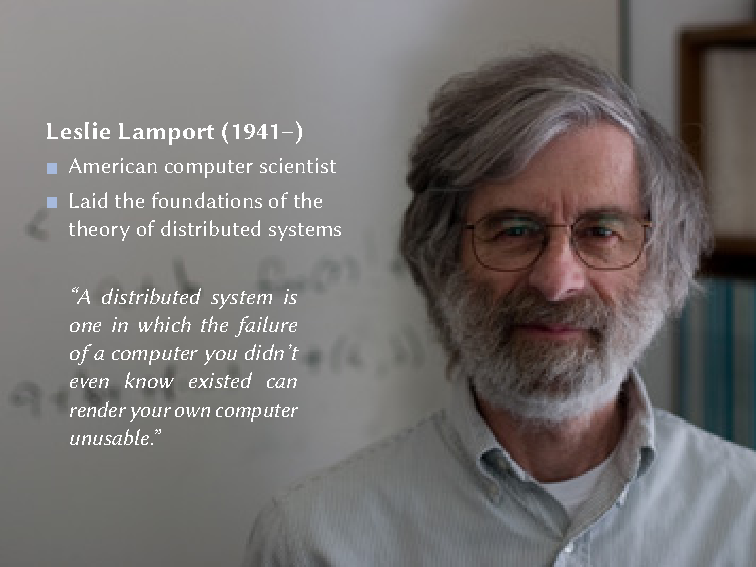
\includegraphics[width=\paperwidth, height=\paperheight, keepaspectratio]{Lecture1/Figures/LL.pdf}};
		\end{tikzpicture}
	}
	\begin{frame}
	\end{frame}
}


\begin{frame}
	\frametitle{Co je \hologo{TeX}}
	\begin{itemize}
		\item \hologo{TeX} je program pro počítačovou sazbu (\emph{computer typesetting system}).
		\item \hologo{TeX} vyslovujeme jako \enquote{tech}. Tři písmena v názvu jsou řecká \enquote{tau-epsilon-chí}. Odvozeno od řeckého \texttau\textepsilon\textchi\textnu\texteta{} [techné], \enquote{umění}, \enquote{dovednost}.
		\item První verze \hologo{TeX}u pochází roku 1978, aktuální 3.141592653 z~ledna 2021.
		\item Zatímco \hologo{LaTeX} je formát dokumentu, \emph{značkovací jazyk}, \hologo{TeX} je \emph{kompilátor}, který překládá zdrojové kódy zapsané v \hologo{LaTeX}u do cílového jazyka, například Pdf.
	\end{itemize}
\end{frame}


{
	\usebackgroundtemplate
	{
		\begin{tikzpicture}[remember picture, overlay]
			\node at (current page.center) {
\includegraphics[width=\paperwidth, height=\paperheight, keepaspectratio]{Lecture1/Figures/DEK.pdf}};
		\end{tikzpicture}
	}
	\begin{frame}
	\end{frame}
}


\begin{frame}
	\frametitle{\hologo{TeX}, \hologo{LaTeX} a okolí}
	\begin{description}
		\item[\hologo{LaTeX}] -- značkovací jazyk (obdoba: jazyk HTML)
		\item[\hologo{TeX}] -- překladač (obdoba: renderovací jádro, lze jich mít víc)
		\item[\hologo{pdfTeX}] -- překladač s přímým výstupem do Pdf,
		\item[\hologo{pdfLaTeX}] -- překladač jazyka \hologo{LaTeX}, postavený nad \hologo{pdfTeX}em
		\item[další překladače]\mbox{}
			\begin{itemize}
				\item \hologo{XeLaTeX} -- nativní podpora UTF-8, přístup k~systémovým fontům,
				\item \hologo{LuaTeX} -- integrace skriptovacího jazyka Lua.
			\end{itemize}
		\item[další programy]\mbox{}
			\begin{itemize}
				\item \hologo{biber}, \hologo{BibTeX} -- zpracování bibliografie,
				\item MakeIndex, xindy -- zpracování rejstříků.
			\end{itemize}
	\end{description}
\end{frame}


\subsection{Proč se učit \hologo{LaTeX}}
\begin{frame}
	\frametitle{Proč se učit \hologo{LaTeX}}
	\begin{columns}[t]
		\begin{column}{0.45\textwidth}
			\begin{block}{Kvalita výstupu}
				\begin{itemize}
					\item sofistikované algoritmy sazby
					\item odvozeno od tradiční typografie
				\end{itemize}
			\end{block}
			\begin{block}{Popularita}
				\begin{itemize}
					\item de-facto norma v~akademickém a~vědeckém světě
				\end{itemize}
			\end{block}
		\end{column}
		\begin{column}{0.48\textwidth}
			\begin{block}{Kvalita software}
				\begin{itemize}
					\item stabilita
					\item rychlost
					\item rozšiřitelnost
					\item vstupním formátem text
					\item mnoho druhů výstupu
				\end{itemize}
			\end{block}
			\begin{block}{Svoboda}
				\begin{itemize}
					\item svobodný software
					\item běží na mnoha platformách
				\end{itemize}
			\end{block}
		\end{column}
	\end{columns}
\end{frame}


\begin{frame}
	\frametitle{Proč se učit \hologo{LaTeX} -- škálovatelnost}
	\begin{center}
		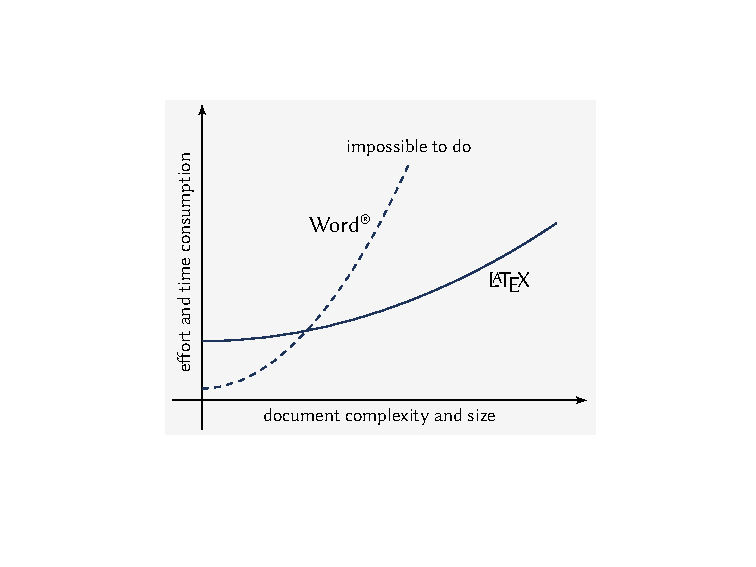
\includegraphics{Lecture1/Figures/Scalability.pdf}\par
		\begin{tiny}
			Převzato z \url{http://www.pinteric.com/miktex.html}
		\end{tiny}
	\end{center}
\end{frame}


\begin{frame}[t]
	\frametitle{Proč se učit \hologo{LaTeX} -- kvalita výstupu}
	\begin{itemize}
		\item Kvalitní sazba a čitelnost
			\begin{itemize}
				\item správné mezery mezi slovy, řádky i odstavci,
				\item kontextově závislé dělení slov,
				\item podpora podřezávání a ligatur.
			\end{itemize}
			\medskip
			\begin{columns}[t]
				\begin{column}{0.45\textwidth}
					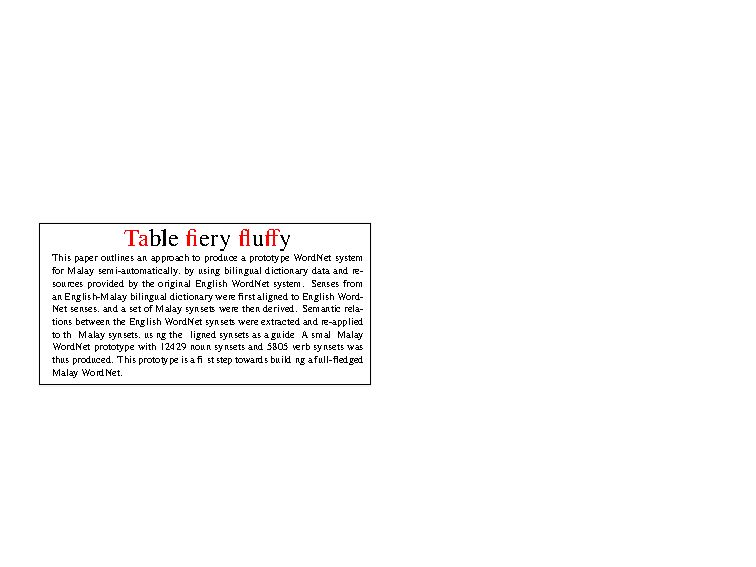
\includegraphics[width=\columnwidth]{Lecture1/Figures/ParagraphSample1.pdf}
				\end{column}
				\begin{column}{0.45\textwidth}
					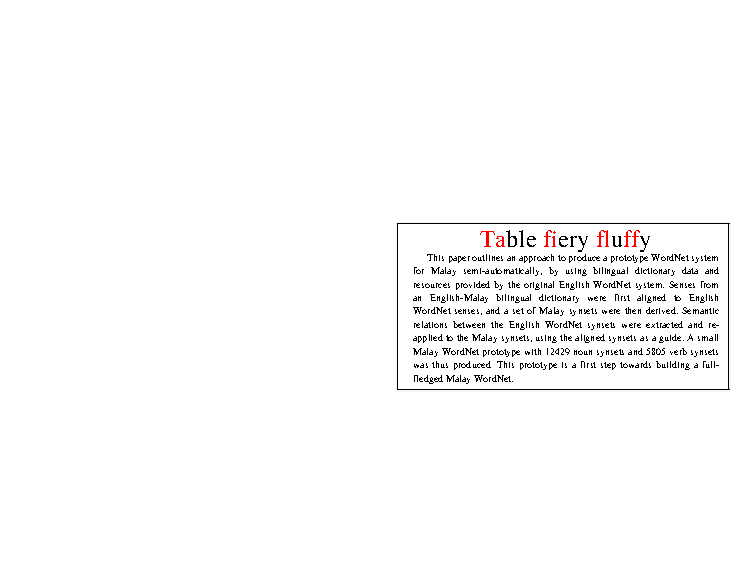
\includegraphics[width=\columnwidth]{Lecture1/Figures/ParagraphSample2.pdf}
				\end{column}
			\end{columns}
		\item Správná matematická sazba
			\begin{columns}[t]
				\begin{column}{0.45\textwidth}
					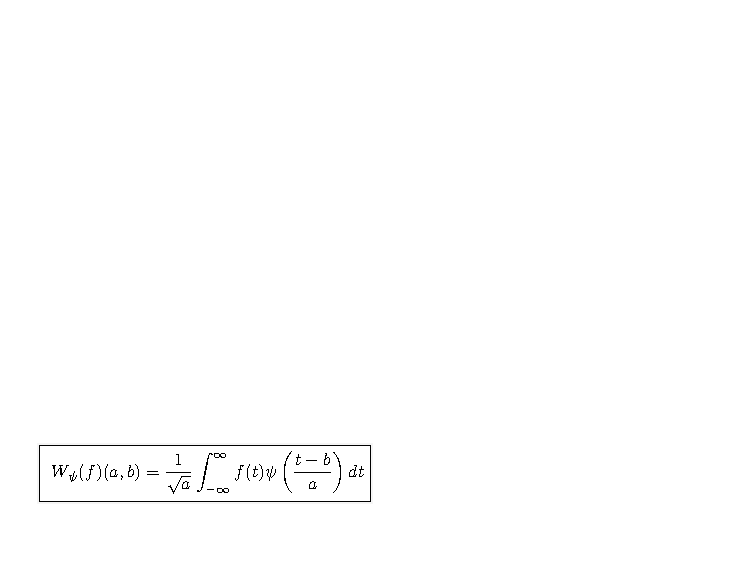
\includegraphics[width=\columnwidth]{Lecture1/Figures/EquationSample1.pdf}
				\end{column}
				\begin{column}{0.45\textwidth}
					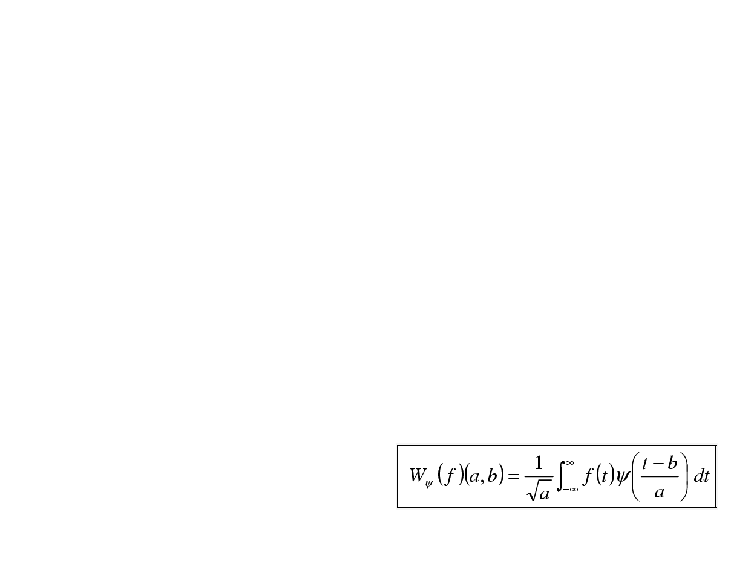
\includegraphics[width=\columnwidth]{Lecture1/Figures/EquationSample2.pdf}
				\end{column}
			\end{columns}
	\end{itemize}
	\begin{center}
		\tiny
		Převzato z \url{http://liantze.penguinattack.org/}.
	\end{center}
\end{frame}


\begin{frame}
	\frametitle{Proč se učit \hologo{LaTeX} -- bakalářská práce}
	\begin{itemize}
		\item Jak jsem posledně formátoval nadpis kapitoly?
		\item Nedával jsem tenhle druh nadpisu kurzívou?
		\item Rovnice se nezobrazuje správně. Někde ano, někde ne!
		\item Do háje, zapomněl jsem aktualizovat obsah dokumentu, nadpisy ani stránky nesedí!
		\item Potřebuji vložit nový obrázek. Jak mám přečíslovat dvacet obrázků?!
		\item Formátování citací a literatury není konzistentní. Jsou pokaždé jiné!
		\item Číslování citací a literatury si neodpovídají!
		\item Editor spadl! \alert{\textbf{Soubor s dokumentem je poškozen! Do pr\ldots!!}} A~zálohu nemám.
	\end{itemize}
\end{frame}


\begin{frame}
	\frametitle{Proč se učit \hologo{LaTeX} -- známé postupy a nástroje}
	\begin{center}
		\emph{Nástroje a postupy používané pro sazbu dokumentů pomocí \hologo{LaTeX}u (\hologo{TeX}u) jsou shodné s~nástroji a postupy používanými pro vývoj software.}
	\end{center}
	\emph{Důležité} -- zdrojový kód dokumentu, obrázky k vložení, konfigurační soubory, atd.\par
	\emph{Nedůležité} -- výsledná podoba dokumentu, vznikne kdykoliv kompilací.\par
	\emph{Známé nástroje a postupy práce} -- dokument jako projekt, správa verzí (Git, Subversion,\ldots), programátorské editory (zvýraznění syntaxe, více otevřených souborů, čistý text), build systémy (např.\ \texttt{make}) nebo integrované vývojové prostředí (IDE).
\end{frame}


\subsection{\hologo{TeX} versus \hologo{LaTeX}}
\begin{frame}
	\frametitle{\hologo{TeX} versus \hologo{LaTeX}}
	\enquote{\emph{Dokument jsem napsal v čistém \hologo{TeX}u.}}
	\begin{itemize}
		\item Virgin \hologo{TeX} -- instrukce sázecího procesoru, \enquote{elementární částice \hologo{TeX}ového vesmíru}, \enquote{nuly a jedničky}.
		\item Čistým \hologo{TeX}em je obvykle míněn formát \hologo{plainTeX}.
		\item \hologo{plainTeX} -- \enquote{assembler}, maximální kontrola nad sazbou dokumentu, ale nutné obrovské předchozí znalosti.
		\item \hologo{LaTeX} -- \enquote{vyšší programovací jazyk}, snadný zápis za cenu jistých omezení (z pohledu \hologo{plainTeX} guru).
		\item Chci \enquote{snadno} napsat technický dokument nebo se \enquote{několik let} učit zvládnout nástroj, kterým dokument psát?
		\item Krásná záminka k tzv.\ flame war.
	\end{itemize}
\end{frame}


\subsection{První dokument v \hologo{LaTeX}u}
\begin{frame}
	\frametitle{První dokument v \hologo{LaTeX}u}
	\begin{enumerate}
		\item V textovém editoru vytvoříme soubor \texttt{FirstDoc.tex} s~následujícím obsahem:\par
			\BVerbatimInput{Samples/FirstDocToInclude.tex}
		\item Na příkazovém řádku spustíme překlad pomocí\\\texttt{pdflatex FirstDoc.tex}
		\item Překladem získáme soubor \texttt{FirstDoc.pdf}
	\end{enumerate}
		\SamplePdfBox{\includegraphics[width=\MaxPdfSampleWidth]{Samples/FirstDoc-crop.pdf}}
\end{frame}


\begin{frame}[fragile]
	\frametitle{První dokument v \hologo{LaTeX}u -- rozbor}
	\BVerbatimInput{Samples/FirstDocToInclude.tex}
	\begin{itemize}
		\item Příkaz |\documentclass| deklaruje \emph{třídu dokumentu}. 
		\item \emph{Preambule} dokumentu
			\begin{itemize}
 				\item oblast mezi |\documentclass| a |\begin{document}|, 
 				\item nastavení parametrů, definice příkazů atd.,
 				\item tato část nesmí generovat viditelný výstup.
			\end{itemize}
		\item Vlastní text dokumentu -- ohraničen |\begin{document}| a~|\end{document}|
	\end{itemize}
\end{frame}


\begin{frame}[fragile]
	\frametitle{První dokument v \hologo{LaTeX}u -- text dokumentu}
	\begin{BVerbatim}
Your first document. This is a very simple example,
with no extra parameters or packages     included.
	\end{BVerbatim}
	\begin{itemize}
		\item Pokud neřekneme jinak, sází \hologo{LaTeX} \emph{odstavce hladkého textu} -- ASCII vstup, zarovnání do bloku, odstavcová zarážka, anglické dělení slov.
		\item Transformace -- konec řádku je nahrazen mezerou, posloupnost mezer je nahrazena jednou mezerou.
		\item Odstavce jsou odděleny aspoň jedním volným řádkem.
	\end{itemize}
	\begin{remark}
		Text dokumentu zapsaný pomocí \hologo{LaTeX}u je zdrojový kód jako každý jiný! Platí jeho úpravu platí obdobná pravidla jako pro každý jiný zdrojový kód, třeba v C++.
	\end{remark}
\end{frame}


\subsection{Distribuce \hologo{TeX}u/\hologo{LaTeX}u}
\begin{frame}[fragile]
	\frametitle{Offline distribuce \hologo{TeX}u/\hologo{LaTeX}u}
	\begin{itemize}
		\item Podobně jako OS Linux, je \hologo{LaTeX} a podpůrný software dostupný ve formě tzv.\ \emph{distribucí}.
		\item Offline distribuce jsou určeny pro lokální instalaci.
	\end{itemize}
	\begin{description}
		\item[\hologo{TeX}Live] -- \url{https://www.tug.org/texlive/}
		\item[Mik\hologo{TeX}] -- \url{https://miktex.org/}
		\item[Mac\hologo{TeX}] -- \url{https://tug.org/mactex/}
	\end{description}
	\begin{block}{Podpora operačních systémů}
		\centering
		\UndefineShortVerb{\|}
		\begin{tabular}{lccc}
			& Windows & Linux & Mac OS\\
			\hline
			\hologo{TeX}Live & \Checkmark & \Checkmark & \XSolidBrush \\
			Mik\hologo{TeX} & \Checkmark & \XSolidBrush & \XSolidBrush \\
			Mac\hologo{TeX} & \XSolidBrush & \XSolidBrush & \Checkmark \\
		\end{tabular}
	\end{block}
\end{frame}


\begin{frame}[fragile]
	\frametitle{Online distribuce \hologo{LaTeX}u}
	\begin{center}
		
\includegraphics[width=0.5\textwidth]{Lecture1/Figures/overleaf_wide_colour_light_bg.pdf}\\
		\url{https://www.overleaf.com/}
	\end{center}
	\begin{itemize}
		\item pro práci je potřebný jen webový prohlížeč a připojení k~internetu,
		\item dokumenty jsou uloženy na serveru Overleaf.com,
		\item snadné sdílení dokumentů,
		\item kolaborativní editace dokumentů,
		\item sledování změn v dokumentu,
		\item integrovaný realtime prohlížeč dokumentů.
	\end{itemize}
\end{frame}


\begin{frame}
	\frametitle{Online distribuce \hologo{LaTeX}u -- pracovní prostředí}
	\begin{center}
		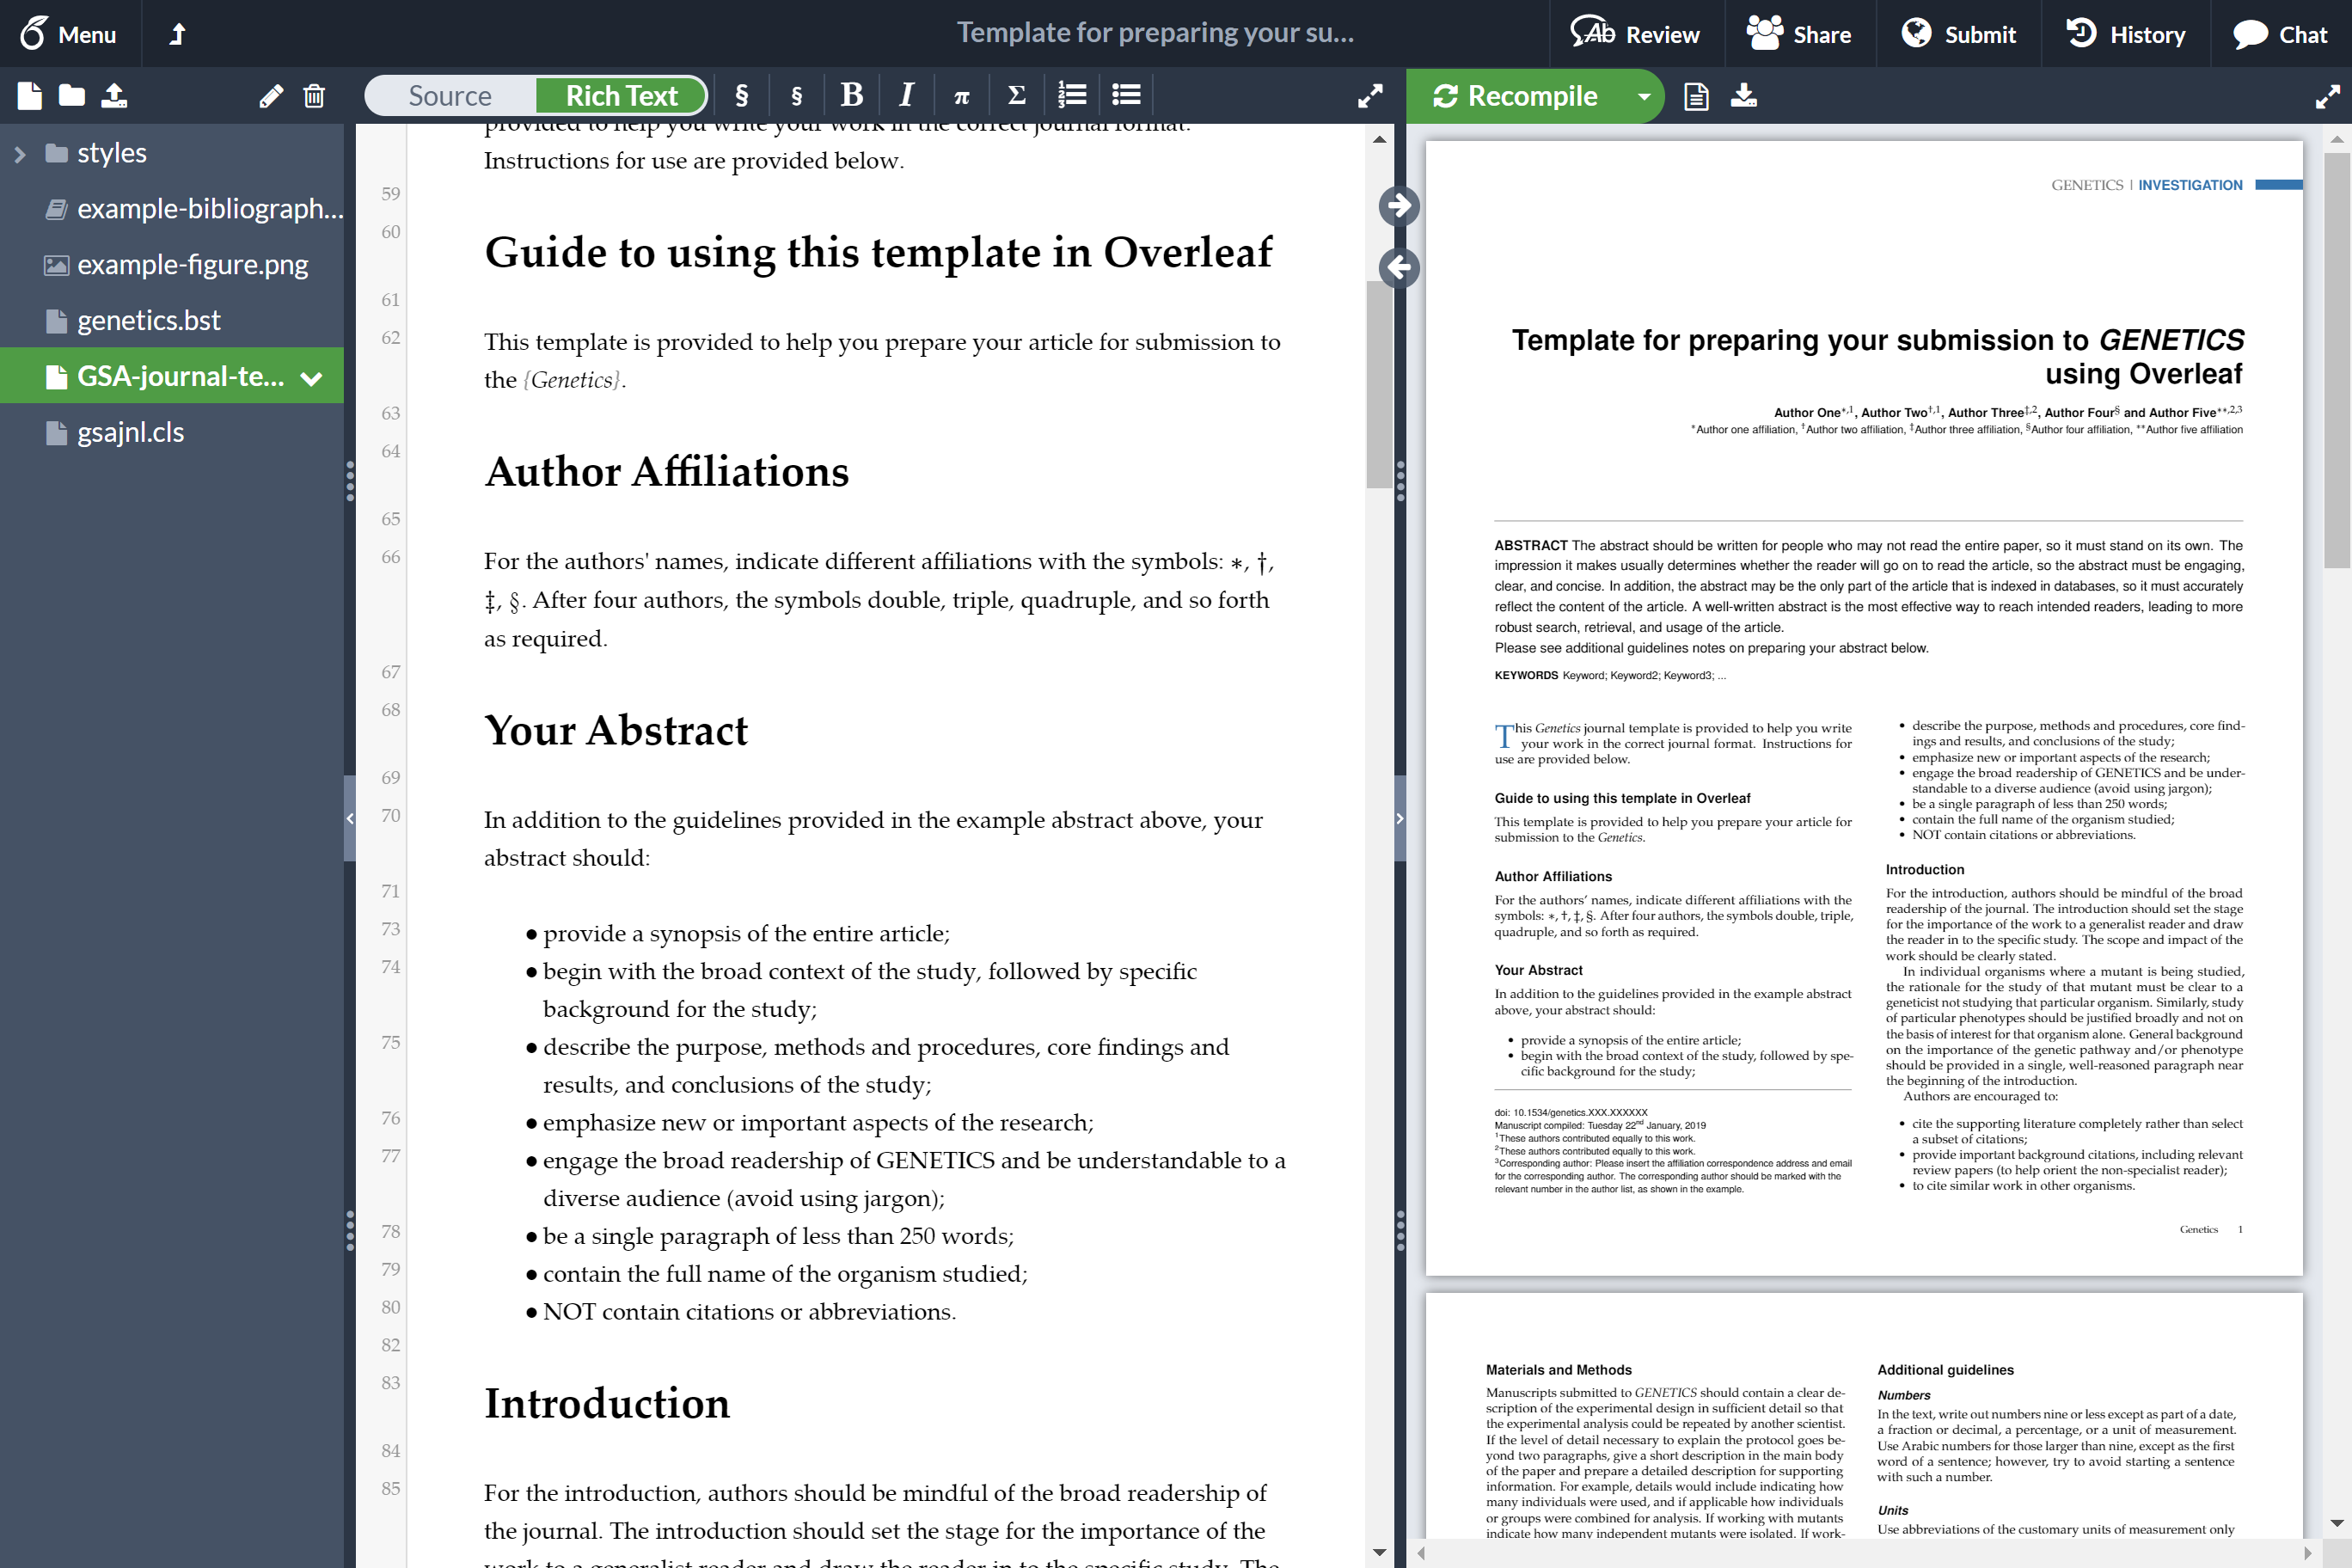
\includegraphics[width=\textwidth]{Lecture1/Figures/Overleaf-journal-template-richtext-example-hires.png}
	\end{center}
\end{frame}


\begin{frame}
	\frametitle{Online distribuce \hologo{LaTeX}u -- sledování změn}
	\begin{center}
		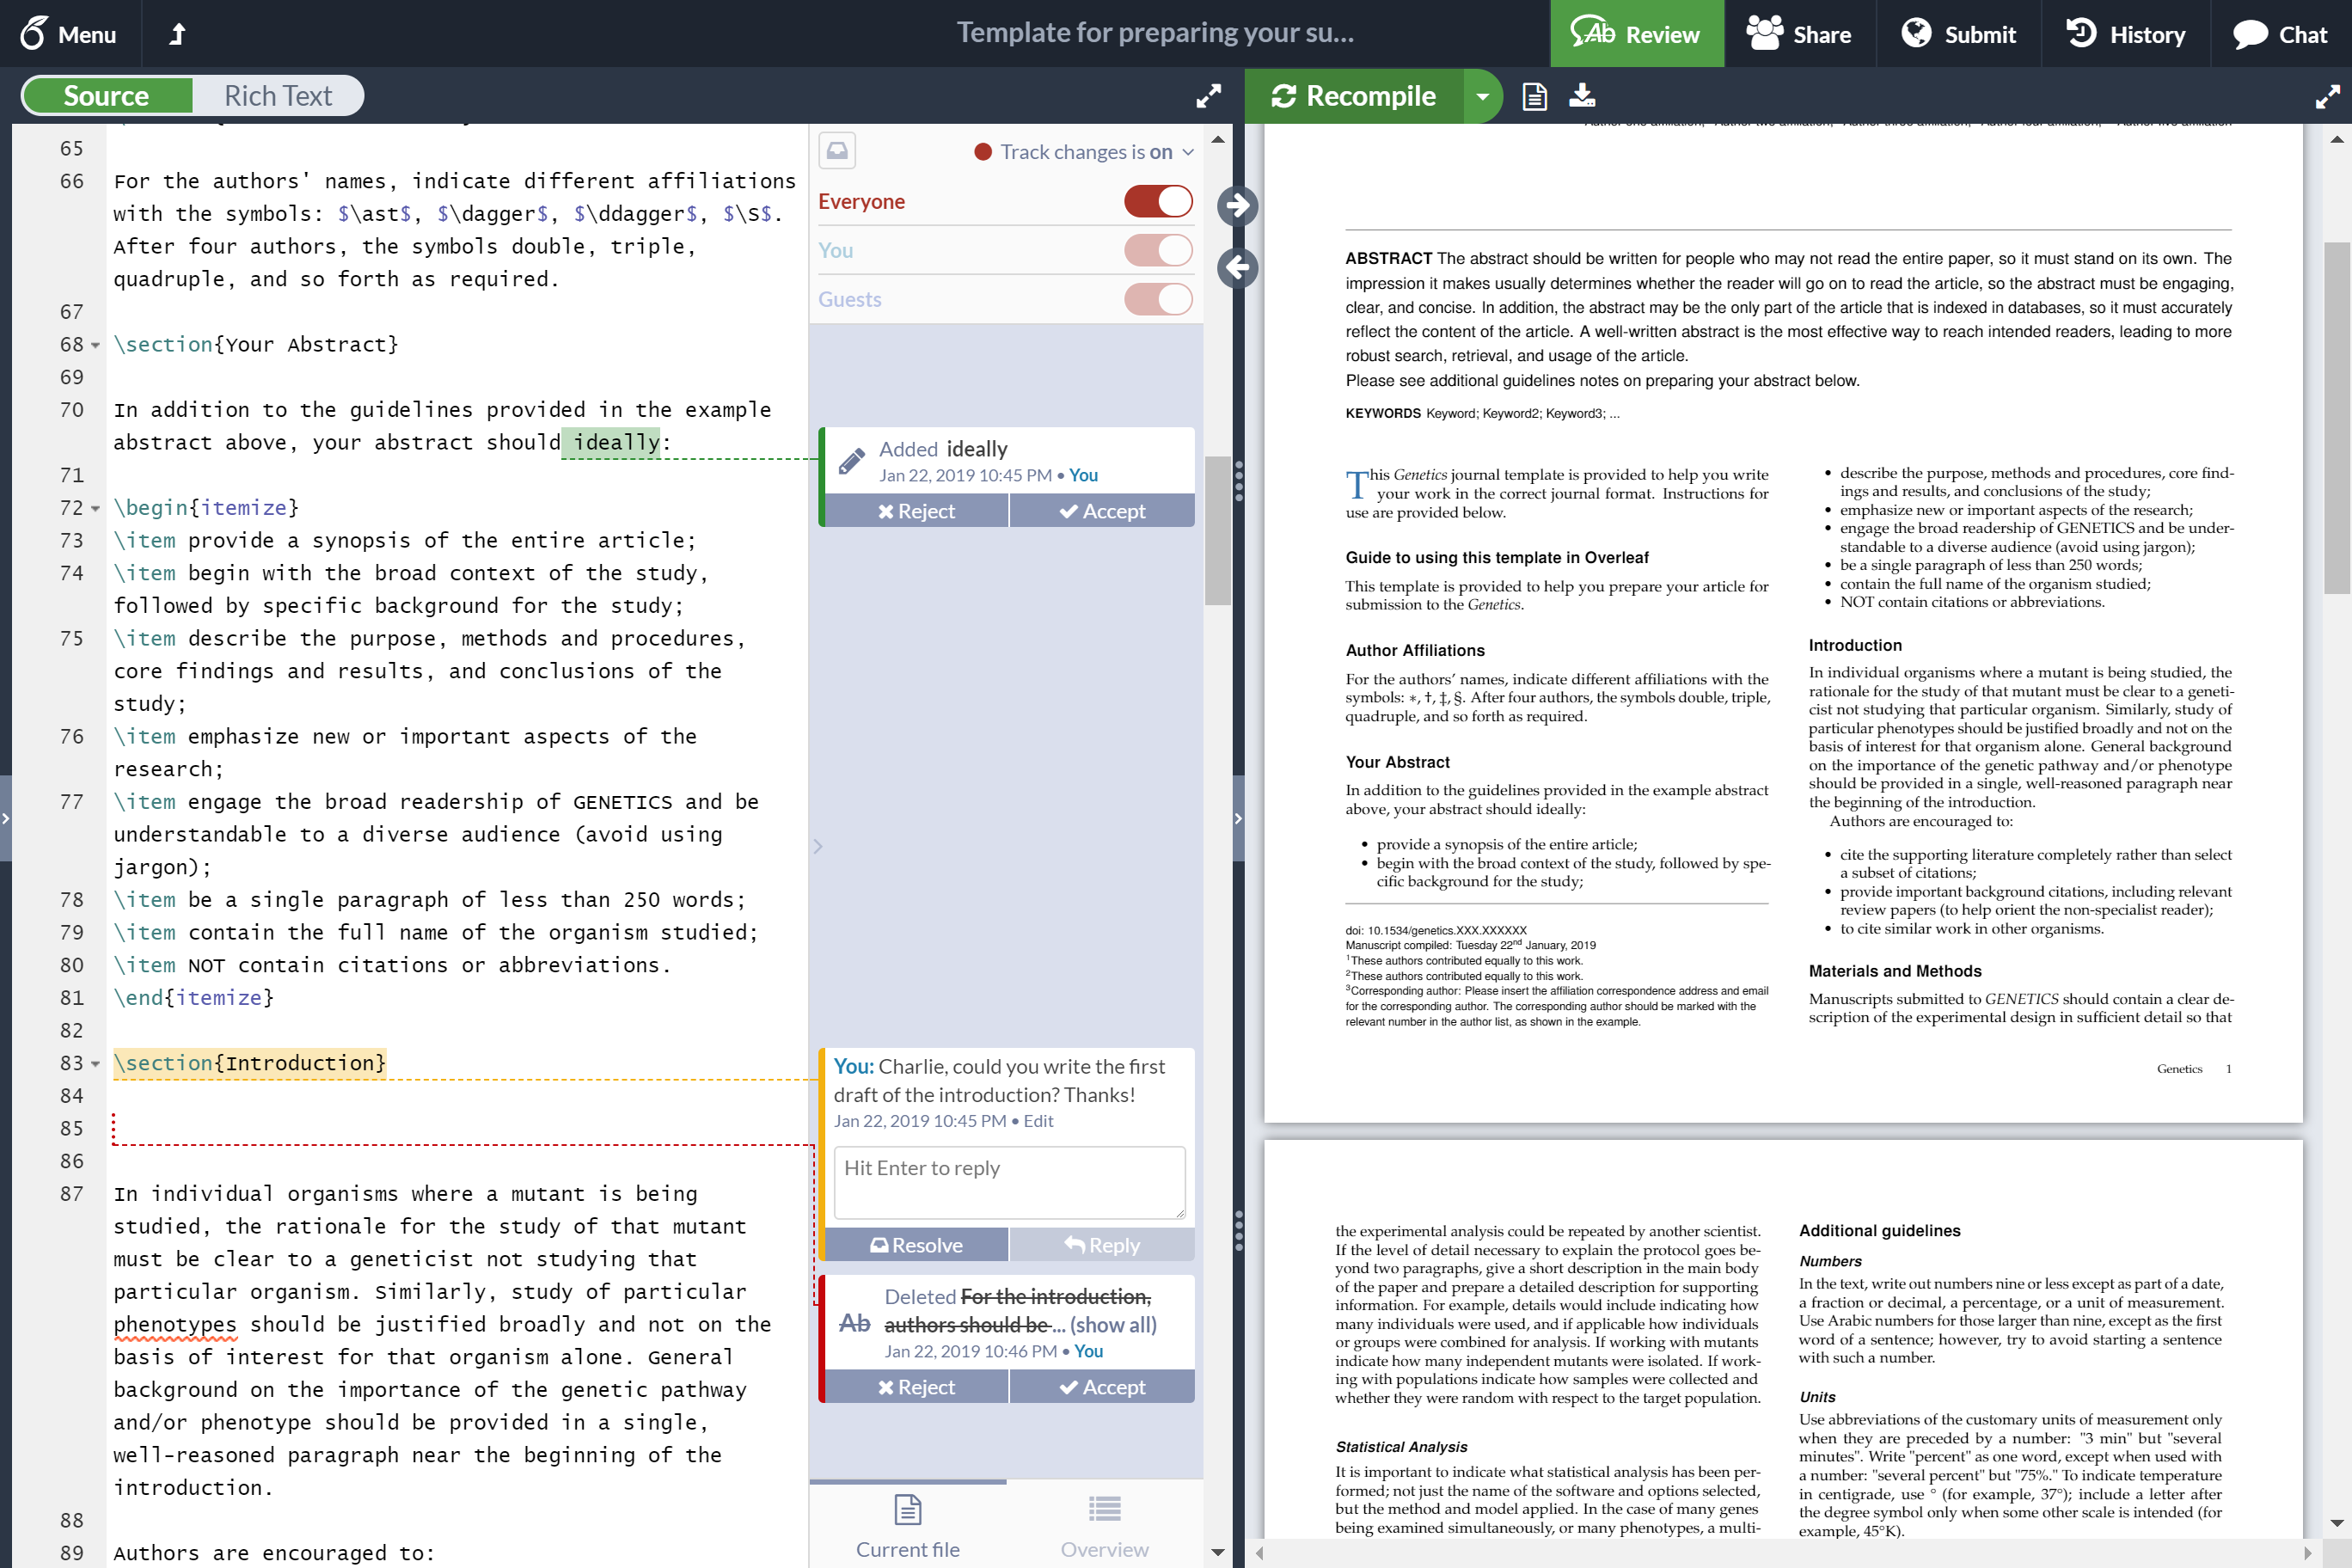
\includegraphics[width=\textwidth]{Lecture1/Figures/Overleaf-journal-template-source-trackchanges-example-hires.png}
	\end{center}
\end{frame}


\begin{frame}
	\frametitle{Overleaf.com -- signalizace chyb při překladu}
	\begin{itemize}
		\item Překladač Overleaf pracuje v tzv.\ \enquote{nonstop} režimu.
		\item Pokud to jen trochu jde, chyby se snaží ignorovat a vysázet dokument za každou cenu. Takový zdrojový kód ale nemusí být bez problémů přeložitelný na jiných systémech.
		\item \alert{Je proto nutné sledovat, zda překlad proběhl bez chyby!}
	\end{itemize}
	\begin{columns}
		\begin{column}{0.45\textwidth}
			\begin{alertblock}{Překlad s chybami}
				\centering
				
\includegraphics[width=0.95\textwidth]{Lecture1/Figures/Overleaf-errors.png}
			\end{alertblock}
		\end{column}
		\begin{column}{0.45\textwidth}
			\begin{block}{Překlad bez chyb}
				\centering
				
\includegraphics[width=0.95\textwidth]{Lecture1/Figures/Overleaf-no-errors.png}
			\end{block}
		\end{column}
	\end{columns}
\end{frame}


\subsection{Editory pro \hologo{LaTeX}}
\begin{frame}
	\frametitle{Editory pro \hologo{LaTeX}}
	\ParagraphCaption{Integrovaná prostředí (IDE)}
	\begin{description}
		\item[Texmaker] -- \url{http://www.xm1math.net/texmaker}
		\item[TeXstudio] -- \url{http://texstudio.sourceforge.net}
		\item[TeXnicCenter] -- \url{https://www.texniccenter.org/}\par{}(v současné době již zastaralé)
	\end{description}
	\ParagraphCaption{Programátorské editory}\par
	Obecně lze použít jakýkoliv programátorský editor - záleží na uživatelově vkusu a zvyku\ldots
	\begin{description}
		\item[Sublime Text] -- \url{http://www.sublimetext.com}
		\item[PSPad]\url{http://www.pspad.com/cz}
	\end{description}
\end{frame}


\subsection{Proces kompilace}
\begin{frame}
	\frametitle{Proces kompilace}
	\begin{center}
		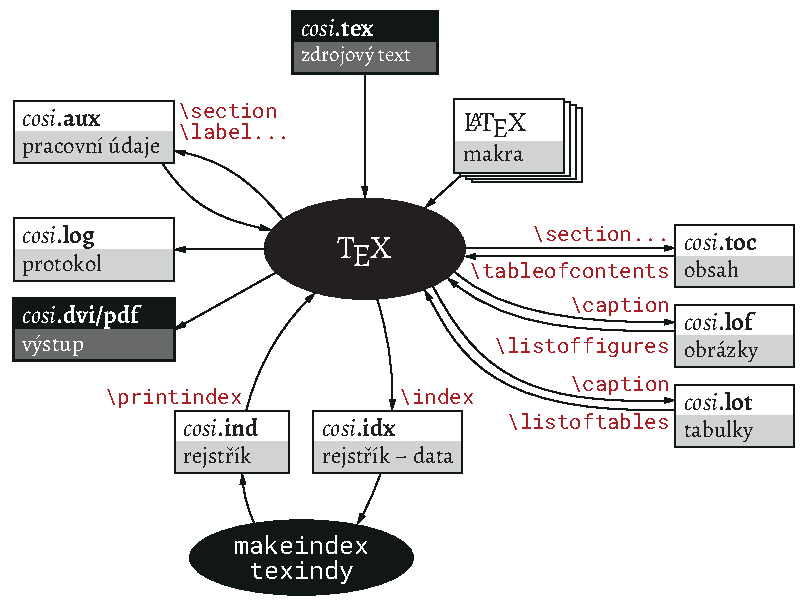
\includegraphics[width=0.85\textwidth]{Lecture1/Figures/CompilationProcess.pdf}
	\end{center}
	{\small{}Převzato z \cite{Satrapa2023}}
\end{frame}


\subsection{Studijní literatura}
\begin{refsection}
	\nocite{Satrapa2023, Kopka2004, Oetiker2011, Oetiker2018, Kopka1999, Lamport1994, Mittelbach2004, Beran2007, Kocicka2004, Felici2003}
	\begin{frame}[t, allowframebreaks]
		\frametitle{Studijní literatura}
		\printbibliography[heading=none]
	\end{frame}
\end{refsection}


\begin{frame}
	\frametitle{Ukázky sazby -- úmluva}
	\begin{itemize}
		\item Předchozí ukázka sazby dokumentu i tato prezentace vznikla za použití \hologo{LaTeX}u.
		\item Je však jasné, že sazba dokumentu na stranu formátu A4 a~sazba prezentace se řídí jinými parametry -- rozměry stránky, použitý font a~jeho velikost, barvy a tak dále.
		\item Pokud nebude výsledek sazby daného typografického prvku v~prezentaci a \enquote{papírovém dokumentu} diametrálně odlišný, bude sazba demonstrována přímo v prezentaci. Ve svém dokumentu však uvidíte sice stejný prvek, ale vysázený pravděpodobně jiným fontem, v jiné barvě a tak dále.
	\end{itemize}
\end{frame}


\begin{frame}[allowframebreaks,fragile]
	\frametitle{Ukázky sazby -- nastavení}
	Ukázky sazby \enquote{papírového dokumentu} probíhají vždy s~následujícím nastavením:\par
	\begin{BVerbatim}
\documentclass[10pt, a4paper]{article}
\usepackage{cmap}
\usepackage[utf8]{inputenc}
\usepackage[T1]{fontenc}
\usepackage{lmodern}
\usepackage[czech]{babel}
\begin{document}
...
\end{document}
	\end{BVerbatim}
	\par
	 Dále mohou být vloženy aktuálně demonstrované balíky maker.\par
	 Překlad probíhá pomocí \hologo{pdfLaTeX}u.
\end{frame}

\endinput

\ThanksAttentionPage

\lecture{Sazba hladkého textu}{lec:PlainText}
\subsection{Struktura zdrojového kódu v \LaTeX{}u}
\begin{frame}
	\frametitle{Struktura zdrojového kódu v \LaTeX{}u}
	\UnderConstruction
\end{frame}


\subsection{Třídy dokumentů}
\begin{frame}
	\frametitle{Třídy dokumentů}
	\UnderConstruction
\end{frame}


\subsection{Externí balíky}
\begin{frame}
	\frametitle{Externí balíky}
	\UnderConstruction
\end{frame}


\subsubsection{Podpora češtiny}
\begin{frame}
	\frametitle{Podpora češtiny}
	\UnderConstruction
\end{frame}


\subsection{Příkazy}
\begin{frame}[fragile]
	\frametitle{Příkazy}
	\begin{itemize}
		\item řídí celou sazbu dokumentu,
		\item slangově se nazývají také \emph{makra},
		\item začínají vždy zpětným lomítkem |\|
		\item rozlišujeme dva typy příkazů:
			\begin{itemize}
				\item \emph{řídící slova} -- tvořená libovolně dlouhou sekvencí písmen anglické abecedy, která je ukončena prvním nepísmenovým znakem.\par
					Pokud je prvním nepísmenovým znakem mezera je řídícím slovem \enquote{sežrána} a zmizí ze vstupu, například:\par
					|\LaTeX{} \LaTeX\ {\LaTeX} logo \LaTeX u|\par \LaTeX{} \LaTeX\ {\LaTeX} logo \LaTeX u
				\item \emph{řídící znaky} -- tvořené jediným nepísmenovým znakem. Například |\#| je řídící znak, který sází znak \#.
			\end{itemize}
	\end{itemize}
\end{frame}


\begin{frame}[fragile]
	\frametitle{Příkazy -- druhy účinku}
	\begin{description}
		\item[Vkládací příkazy] -- do místa svého výskytu vloží danou typografickou konstrukci, například logo |\LaTeX|
		\item[Přepínače] -- změní určitý parametr sazby. Ukončení změny -- konec aktuální skupiny nebo změna daného parametru jiným příkazem.\par
			Např.\ |\itshape| \textit{přepne až do odvolání na kurzívu, zatímco }|\upshape| vrací běžné vzpřímené písmo\ldots
	
		\item[Příkazy s parametrem] -- vytvoří určitou konstrukci za použití daného parametru. Parametry jsou každý zvlášť uzavřeny do složených závorek. Nepovinný parametr se uvádí v hranatých závorkách, před ostatními parametry. Příklad
		|\documentclass[10pt, a4paper]{article}|
	\end{description}
\end{frame}


\subsection{Znaky}
\begin{frame}[fragile]
	\frametitle{Znaky}
	\ParagraphCaption{Sazba \enquote{běžných} znaků}
	\begin{itemize}
		\item deklarace správného kódování v balíku |inputenc|,
		\item vstup znaků přímo z klávesnice,
		\item nejčastěji užívané kódování UTF-8 řeší většinu problémů,
		\item ale mohou nastat situace, kdy jej nelze použít.
	\end{itemize}
\end{frame}


\begin{frame}[fragile]
	\frametitle{Znaky -- méně běžné znaky}
	\begin{itemize}
		\item Akcentované znaky
			\begin{center}
				\begin{tabular}{*{8}{c}}
					|\'{o}| & \'{o} & |\`{o}| & \`{o} & |\"{o}| & \"{o} & |\H{o}| & \H{o}\\
					|\v{e}| & \v{e} & |\u{o}| & \u{o} & |\^{o}| & \^{o} & |\~{o}| & \~{o}\\
					|\c{c}| & \c{c} & |\k{a}| & \k{a} & |\={o}| & \={o} & |\b{o}| & \b{o}\\
					|\.{c}| & \.{c} & |\d{c}| & \d{c} & |\r{a}| & \r{a} & |\t{oo}| & \t{oo}\\
				\end{tabular}
			\end{center}
		\item Mezinárodní znaky
			\begin{center}
				\begin{tabular}{*{8}{c}}
					|\oe| & \oe & |\OE| & \OE & |\ae| & \ae & |\AE| & \AE\\
					|\o| & \o & |\O| & \O & |\aa| & \aa & |\AA| & \AA\\
					|\l| & \l & |\L| & \L & |\ss| & \ss & |\SS| & \SS\\
				\end{tabular}
			\end{center}
	\end{itemize}
\end{frame}


\begin{frame}[fragile]
	\frametitle{Znaky -- ostatní symboly}
		\begin{itemize}
			\item Standardní \hologo{LaTeX}
				\begin{center}
					\begin{tabular}{*{6}{c}}
						|\copyright| & \copyright & |\S| & \S & |\ldots| & \ldots\\
						|\textregistered| & \textregistered & |\P| & \P & |\pounds| & \pounds\\
					\end{tabular}
				\end{center}
			\item Externí balíky
				\begin{center}
					\begin{tabular}{lcl}
						|\usepackage{textcomp}| & |\textdegree| & -5\textdegree{}C\\
						|\usepackage[official]{eurosym}| & |\euro| & \euro{}50\\
					\end{tabular}
				\end{center}
		\end{itemize}
		\medskip
		Kompletní přehled symbolů \hologo{LaTeX}u lze nalézt v \cite{Pakin2017}.
\end{frame}


\begin{frame}[fragile]
	\frametitle{Znaky -- ostatní symboly}
	\begin{center}
		\begin{tabular}{cll}
			\textbackslash & zahajuje příkazy & |\textbackslash|\\
			\{ \} & vymezují skupiny & |\{| a |\}|\\
			\& & odděluje sloupce tabulky & |\&|\\
			\% & zahajuje komentář & |\%|\\
			\textasciitilde & nezlomitelná mezera & |\textasciitilde|\\
			\$ & zahajuje/ukončuje matemat.\ režim & |\$|\\
			\# & odkaz na parametr makra & |\#|\\
			\textasciicircum & horní index & |\textasciicircum|\\
			\_ & dolní index & |\_|\\
		\end{tabular}
	\end{center}
\end{frame}


\begin{frame}[fragile]
	\frametitle{Znaky aneb nelze pomlčet o pomlčkách}
	V typografii existují tři druhy pomlček:
	\begin{description}
		\item[spojovník] -- krátká, silná pomlčka, používaná pro dělení slov, zvratné \enquote{-li} a složená slova
		\item[pomlčka] -- pomlčka ve větách a
		\item[dlouhá pomlčka] -- v americké typografii.
	\end{description}
	\begin{center}
		\begin{tabular}{l@{\hspace{3em}}c@{\hspace{3em}}c}
			Druh pomlčky & & Zápis v \hologo{LaTeX}u\\
			\hline
			Spojovník & - & |-|\\
			Pomlčka & -- & |-||-|\\
			Dlouhá pomlčka & --- & |-||-||-|\\
		\end{tabular}
	\end{center}
\end{frame}


\subsection{Skupiny a prostředí}
\begin{frame}
	\frametitle{Skupiny a prostředí}
	\UnderConstruction
\end{frame}


\subsection{Odstavce a odřádkování}
\begin{frame}
	\frametitle{Odstavce a odřádkování}
	\UnderConstruction
\end{frame}


\begin{frame}
	\frametitle{Sazba na levý praporek}
	\BVerbatimInput{Samples/FlushLeftToInclude.tex}
	\bigskip
	\SamplePdfBox{\includegraphics{Samples/FlushLeft-crop.pdf}}
\end{frame}


\begin{frame}
	\frametitle{Sazba na pravý praporek}
	\BVerbatimInput{Samples/FlushRightToInclude.tex}
	\bigskip
	\SamplePdfBox{\includegraphics{Samples/FlushRight-crop.pdf}}
\end{frame}


\begin{frame}
	\frametitle{Sazba na střed}
	\centering
	\BVerbatimInput{Samples/CenteredTextToInclude.tex}
	\bigskip
	\SamplePdfBox{\includegraphics{Samples/CenteredText-crop.pdf}}
\end{frame}


\subsection{Komentáře}
\begin{frame}[fragile]
	\frametitle{Komentáře}
	\begin{itemize}
		\item Komentáře ve zdrojovém kódu dokumentu zapisujeme pomocí znaku |%|.
		\item \hologo{LaTeX} ignoruje vše od znaku |%| do konce řádku.
		\item Víceřádkové komentáře standardně neexistují, lze ale použít prostředí |comment| z balíku maker |verbatim|.
	\end{itemize}
	\medskip
	\BVerbatimInput{Samples/CommentSampleToInclude.tex}
	\medskip
	\SamplePdfBox{\includegraphics[width=\textwidth]{Samples/CommentSample-crop.pdf}}
\end{frame}


\subsection{Seznamy}
\begin{frame}[fragile]
	\frametitle{Seznamy}
	\begin{itemize}
		\item \LaTeX{} zahrnuje tři druhy seznamů:
			\begin{itemize}
				\item s odrážkami tj.\ nečíslované,
				\item číslované a
				\item s nadpisy.
			\end{itemize}
		\item Jednotlivé položky jsou označeny makrem |\item|.
		\item Seznamy lze vzájemně vnořovat.\par
		\item Jsou k dispozici, nezávisle na sobě, 4 úrovně nečíslovaných a 4 úrovně číslovaných seznamů.
	\end{itemize}
\end{frame}


\begin{frame}[fragile]
	\frametitle{Seznam s odrážkami}
	\BVerbatimInput{Samples/ItemizeToInclude.tex}
	\SamplePdfBox{\includegraphics{Samples/Itemize-crop.pdf}}
\end{frame}


\begin{frame}[fragile]
	\frametitle{Číslovaný seznam}
	\BVerbatimInput{Samples/EnumerateToInclude.tex}
	\SamplePdfBox{\includegraphics{Samples/Enumerate-crop.pdf}}
\end{frame}


\begin{frame}[fragile]
	\frametitle{Seznam s nadpisy}
	\BVerbatimInput[commandchars=+`']{Samples/DescriptionToInclude.tex}
	\SamplePdfBox{\includegraphics{Samples/Description-crop.pdf}}
\end{frame}


\begin{frame}[fragile]
	\frametitle{Vnořené seznamy -- nečíslované}
	\centering
	\begin{tabular}{cc}
		\SamplePdfBox{\includegraphics{Samples/NestedItemize-crop.pdf}}&
		\BVerbatimInput[boxwidth=0.6\MaxPdfSampleWidth]{Samples/NestedItemizeToInclude.tex}\\
	\end{tabular}
\end{frame}


\begin{frame}[fragile]
	\frametitle{Vnořené seznamy -- číslované}
	\centering
	\begin{tabular}{cc}
		\SamplePdfBox{\includegraphics{Samples/NestedEnumerate-crop.pdf}}&
		\BVerbatimInput[boxwidth=0.65\MaxPdfSampleWidth]{Samples/NestedEnumerateToInclude.tex}\\
	\end{tabular}
\end{frame}


\subsection{Písmo}
\begin{frame}
	\frametitle{Písmo}
	V současnosti je práce s písmem založena na \emph{New Font Selection Scheme} (NFSS), které definuje čtyři základní charakteristiky písma:
	\begin{itemize}
		\item rodina
		\item duktus
		\item tvar
		\item stupeň
	\end{itemize}
	Charakteristiky jsou navzájem nezávislé, nastavení písma si lze představit jako bod ve 4D prostoru -- jedna osa je rodina, druhá duktus\ldots
\end{frame}


\begin{frame}[fragile]
	\frametitle{Písmo}
	\ParagraphCaption{Rodina (family)}
	\begin{itemize}
		\item Určuje základní charakter písma
		\item Rozlišujeme tři rodiny a jim odpovídající příkazy:
	\end{itemize}
	\begin{center}
		\begin{tabular}{cl}
			|\rmfamily| & antikva (písmo serifové, anglicky \textrm{RoMan})\\
			|\sffamily| & grotesk (písmo bezserifové, \textsf{Sans seriF})\\
			|\ttfamily| & písmo neproporcionální (\texttt{TypewriTer})\\
		\end{tabular}
	\end{center}
	\ParagraphCaption{Duktus (series)}
	\begin{itemize}
		\item specifikuje tloušťku jednotlivých tahů v písmu
	\end{itemize}
	\begin{center}
		\begin{tabular}{cl}
			|\mdseries| & běžné písmo (MeDium)\\
			|\bfseries| & tučné písmo (\textbf{BoldFace})\\
		\end{tabular}
	\end{center}
\end{frame}


\begin{frame}[fragile]
	\frametitle{Písmo -- tvar (shape)}
	Specifikuje tvarovou variantu písma
	\begin{center}
		\begin{tabular}{cl}
			|\upshape| & běžné vzpřímené písmo\\
			|\itshape| & kurzíva (\textit{ITalics})\\
			|\slshape| & skloněné písmo (\textsl{SLanted})\\
			|\scshape| & kapitálky (\textsc{Small Capitals})\\
		\end{tabular}
	\end{center}
	\begin{remark}
		\begin{enumerate}
			\item Kurzíva, na rozdíl od skloněného písma, nemá jen skloněnou svislou osu, ale má i jinou kresbu písmen, např.\ \textrm{\huge{}a} vs. \textit{\huge{}a}.
			\item Většina fontů nemá skloněné písmo tj.\ |\slshape| přepne na kurzívu.
		\end{enumerate}
	\end{remark}
\end{frame}


\begin{frame}[fragile]
	\frametitle{Písmo -- stupeň (size)}
	Určuje relativní velikost písma vůči |\normalsize|, která je uvedena v~hlavičce dokumentu.
	\begin{center}
		\begin{tabular}{cl}
			|\tiny| & {\tiny{}nejmenší}\\
			|\scriptsize| & {\scriptsize{}velikost horního a dolního indexu}\\
			|\footnotesize| & {\footnotesize{}velikost poznámek pod čarou}\\
			|\small| & {\small{}malé písmo}\\
			|\normalsize| & {\normalsize{}normální velikost}\\
			|\large| & {\large{}větší písmo}\\
			|\Large| & {\Large{}ještě větší}\\
			|\LARGE| & {\LARGE{}opravdu velké}\\
			|\huge| & {\huge{}skoro největší}\\
			|\Huge| & {\Huge{}největší}\\
		\end{tabular}
	\end{center}
\end{frame}


\subsection{Struktura dokumentu}
\begin{frame}[fragile]
	\frametitle{Struktura dokumentu}
	\begin{itemize}
		\item Většina dokumentů je členěna do hierarchické struktury kapitol, sekcí atd.
		\item Kapitoly jsou obvykle číslovány, zařazeny do obsahu dokumentu.
		\item \emph{Nadpisy stejné úrovně musí vypadat stejně}!
		\item \hologo{LaTeX} poskytuje až 7 úrovní strukturování dokumentu.
	\end{itemize}
	Makra mají jednotný tvar
	\begin{Verbatim}
\section_macro_name[krátký nadpis]{nadpis}
	\end{Verbatim}
	Nepovinný |krátký nadpis| většinou chybí.
\end{frame}

\begin{frame}[fragile]
	\frametitle{Struktura dokumentu -- makra pro členění dokumentu}
	\begin{center}
		\begin{tabular}{clccc}
			& & \multicolumn{3}{c}{Třída dokumentu}\\
			Úroveň & Makro & |article| & |report| & |book|\\
			\hline
			-1 & |\part| & \XSolidBrush & \multicolumn{2}{c}{volitelně}\\
			 0 & |\chapter| & \XSolidBrush & \Checkmark & \Checkmark \\
			 1 & |\section| & \Checkmark & \Checkmark & \Checkmark\\
			 2 & |\subsection| & \Checkmark & \Checkmark & \Checkmark\\
			 3 & |\subsubsection| & \Checkmark & \Checkmark & \Checkmark \\
			 4 & |\paragraph| & \Checkmark & \Checkmark & \Checkmark\\
			 5 & |\subparagraph| & \Checkmark & \Checkmark & \Checkmark\\
		\end{tabular}
	\end{center}
\end{frame}


\begin{frame}[fragile]
	\frametitle{Struktura dokumentu -- funkcionalita maker}
	Makra pro sazbu kapitol provádí celou řadu činností:
	\begin{enumerate}
		\item Vygeneruje číslo dané části textu. V hierarchii kapitol se \emph{nesmí přeskakovat} -- vynecháním úrovně dostaneme v~číslování kapitol nuly!
		\item Vysází číslo kapitoly a |nadpis| stylem odpovídajícím dané úrovni nadpisu. Styl definuje písmo, místo před nadpisem, za nadpisem, přechod na na novou stránku atd.
		\item Vloží číslo kapitoly, |nadpis| a číslo stránky do obsahu.Pokud je uveden |krátký nadpis| je do obsahu vložen |krátký nadpis|. V textu je pochopitelně ale vysázen |nadpis|.
		\item Upraví záhlaví stránky, pokud je použito tzv.\ živé záhlaví. I~zde se přednostně uplatní |krátký nadpis|.
	\end{enumerate}
\end{frame}


\begin{frame}[fragile]
	\frametitle{Struktura dokumentu -- omezené verze maker}
	Ke všem makrům od |\part| po |\subparagraph| existují omezené verze
	\begin{Verbatim}
\section_macro_name*{nadpis}
	\end{Verbatim}
	Tato makra provedou pouze krok 2 z předchozího seznamu -- vysází |nadpis| požadovaným stylem.
	\begin{example}
		Předmluva v knize -- chceme nadpis \enquote{Předmluva} vysázet jako kapitolu, ale není nutné aby byla v obsahu.
	\begin{Verbatim}
\chapter*{Předmluva}
Vážení čtenáři dostává se Vám do rukou...
	\end{Verbatim}
	\end{example}
\end{frame}


\subsection{Obsah dokumentu}
\begin{frame}[allowframebreaks, fragile]
	\frametitle{Obsah dokumentu}
	\begin{itemize}
		\item Na požadované místo v dokumentu uvedeme makro |\tableofcontents|.
		\item Položky obsahu se automaticky vytvoří z nadpisů použitých v makrech pro členění dokumentu.
		\item Obsah dokumentu je sestavován v pomocném |toc| souboru, který obsahuje nadpisy kapitol, jejich čísla a čísla odpovídajících stran.
	\end{itemize}
\end{frame}


\begin{frame}[allowframebreaks, fragile]
	\frametitle{Sestavení obsahu dokumentu}
	Vytvoření obsahu vyžaduje \emph{nejméně dva překlady} \hologo{LaTeX}em:
	\begin{description}
		\item [1. překlad] -- |toc| soubor neexistuje, makro |\tableofcontents| vytvoří jen nadpis \enquote{Obsah}. Při překladu dokumentu je postupně vytvářen |toc| soubor.
		\item [2. překlad] -- makro |\tableofcontents| načte |toc| soubor vytvořený při předchozím překladu a sestaví z něj obsah dokumentu. Nicméně |toc| soubor je vytvářen i~v~tomto překladu.
	\end{description}
	\begin{remarks}
		\begin{enumerate}
			\item Je zřejmé, že vytváření obsahu je zpožděno o \enquote{jedno kolo} za textem dokumentu.
			\item Pokud chceme obsah aktualizovat, např.\ po změně nadpisu, musíme opět provést dva překlady.
			\item V závislosti na umístění obsahu dokumentu může být nutný i třetí překlad. Pokud je obsah umístěn před samotným textem dokumentu, může dojít vložením obsahu dokumentu k posunutí čísel stran.
		\end{enumerate}
	\end{remarks}
\end{frame}


\begin{frame}[allowframebreaks, fragile]
	\frametitle{Seznam obrázků a tabulek}
	Do dokumentu lze vložit také
	\begin{itemize}
		\item seznam obrázků -- |\listoffigures| a
		\item seznam tabulek -- |\listoftables|.
	\end{itemize}
	Seznam obrázků a tabulek vzniká zcela identickým mechanismem jako obsah dokumentu s tím rozdílem, že:
	\begin{itemize}
		\item položky obou seznamů se berou z maker |\caption| v~prostředí |figure|, respektive |table| a
		\item místo |toc| souboru se používají |lof| (list of figures) a |lot| (list of tables) soubory.
	\end{itemize}
\end{frame}


\subsection{Křížové odkazy}
\begin{frame}
	\frametitle{Křížové odkazy}
	\UnderConstruction
\end{frame}


\subsection{Poznámky}
\begin{frame}[fragile]
	\frametitle{Poznámky -- poznámky pod čarou}
	\BVerbatimInput{Samples/FootnoteSampleToInclude.tex}
	\SamplePdfBox{\includegraphics{Samples/FootnoteSample-crop.pdf}}
	\begin{remark}
		Pokud nelze vytvořit poznámku pod čarou přímo (např.\ v~tabulkách) použijeme |\footnotemark| pro sazbu značky a~následně |\footnotetext{text poznámky}| pro vlastní sazbu poznámky.
	\end{remark}
\end{frame}


\begin{frame}[fragile]
	\frametitle{Poznámky -- poznámky na okraji}
	\BVerbatimInput{Samples/MarginparnoteSampleToInclude.tex}
	\SamplePdfBox{\includegraphics{Samples/MarginparnoteSample-crop.pdf}}
	Poznámka na okraji se sází na boční okraj vedle řádku na kterém se objevil příkaz |\marginpar|.
	U jednostranné sazby se poznámka vysází na pravý okraj, u oboustranné na vnější okraje.
\end{frame}


\subsection{Další externí balíky}
\begin{frame}
	\frametitle{Externí balíky}
	\UnderConstruction
\end{frame}


\subsubsection{Hypertextové odkazy}
\begin{frame}
	\frametitle{Hypertextové odkazy}
	\UnderConstruction
\end{frame}


\subsubsection{Uvozovky}
\begin{frame}
	\frametitle{Uvozovky}
	\UnderConstruction
\end{frame}


\subsubsection{Užitečné balíky maker}
\begin{frame}
	\frametitle{Užitečné balíky maker}
%	enumitem -- změna vzhledu seznamů
	\UnderConstruction
\end{frame}


\subsection{Časté chyby}
\begin{frame}
	\frametitle{Časté chyby}
	\UnderConstruction
\end{frame}


\subsection{Správa velkých projektů}
\begin{frame}
	\frametitle{Správa velkých projektů}
	\UnderConstruction
\end{frame}

\endinput
\ThanksAttentionPage

\lecture{Sazba matematiky}{lec:Mathematics}
\begin{frame}
	\frametitle{Sazba matematiky}
	\begin{itemize}
		\item Matematická sazba je integrální součástí \TeX{}u -- nekvalitní matematická sazba byla i jednou z příčin jeho vzniku.
		\item \LaTeX{} ke schopnostem \TeX{}u přidává několik zastřešujících konstrukcí.
		\item Matematika je v \LaTeX{}u zapisována pomocí speciální syntaxe, která je navržena
			\begin{enumerate}
				\item pro pohodlný vstup z klávesnice a
				\item pro snadné čtení zdrojového kódu dokumentu.
			\end{enumerate}
	\end{itemize}
\end{frame}


\begin{frame}
	\frametitle{Sazba matematiky -- první ukázka}
	\BVerbatimInput[boxwidth=\MaxPdfSampleWidth]{Samples/MathSampleToInclude1.tex}
	\SamplePdfBox{\includegraphics[width=\MaxPdfSampleWidth]{Samples/MathSample1-crop.pdf}}
\end{frame}


\subsection{Režimy sazby matematiky}
\begin{frame}
	\frametitle{Režimy sazby matematiky}
	Sazba matematiky probíhá ve dvou režimech:
	\begin{description}
		\item [inline] -- matematické formule jsou součástí odstavce; sazba je kompaktní ve svislém směru aby co nejméně ovlivňovala samotný odstavec.
		\item [display] -- formule jsou sázeny na střed na samostatné řádky.
	\end{description}
\end{frame}


\begin{frame}[fragile]
	\frametitle{Inline režim}
	\BVerbatimInput[boxwidth=\MaxPdfSampleWidth]{Samples/MathSampleToInclude2.tex}
	\SamplePdfBox{\includegraphics[width=\MaxPdfSampleWidth]{Samples/MathSample2-crop.pdf}}
	Pro označení lze použít:
	\begin{itemize}
		\item prostředí |math|, čili konstrukci |\begin{math}|\ldots|\end{math}|
		\item dvojici znaků |\(| před a dvojici znaků |\)| za vzorcem
		\item jeden znak |$| před a jeden znak |$| za vzorcem.
	\end{itemize}
	Všechny tři způsoby jsou navzájem ekvivaletní.
\end{frame}


\begin{frame}[allowframebreaks, fragile]
	\frametitle{Display režim}
	\BVerbatimInput[boxwidth=\MaxPdfSampleWidth]{Samples/MathSampleToInclude3.tex}
	\SamplePdfBox{\includegraphics[width=\MaxPdfSampleWidth]{Samples/MathSample3-crop.pdf}}
	\framebreak
	Display režim má dvě formy:
	\begin{description}
		\item [nečíslovanou] -- pro označení lze použít prostředí |displaymath| nebo |\[|\ldots|\]| či |$$|\ldots|$$|
		\item [číslovanou] -- prostředí |equation|.
	\end{description}
\end{frame}


\subsection{Řecká písmena a matematické symboly}
\begin{frame}
	\frametitle{Zápis matematické symboliky}
	V matematických formulích se vyskytují symboly, které není možné zapsat přímo z klávesnice. Tyto symboly se zapisují pomocí speciálních maker. Jde především o tyto symboly:
	\begin{itemize}
		\item řecká písmena,
		\item šipky,
		\item binární a relační operátory a
		\item některé další symboly.
	\end{itemize}
\end{frame}


\begin{frame}[fragile]
	\frametitle{Řecká písmena}
	\begin{center}
		\begin{tabular}{clcl}
			$\alpha A$ &|\alpha A| & $\nu N$ & |\nu N|\\
			$\beta B$ & |\beta B| & $\xi \Xi$ & |\xi \Xi|\\
			$\gamma \Gamma$ & |\gamma \Gamma| & $oO$ & |o O|\\
			$\delta \Delta$ & |\delta \Delta| & $\pi \Pi$ & |\pi \Pi|\\
			$\epsilon \varepsilon E$ & |\epsilon \varepsilon E| & $\rho \varrho P$ & |\rho\varrho P|\\
			$\zeta Z$ & |\zeta Z| & $\sigma \Sigma$ & |\sigma \Sigma|\\
			$\eta H$ & |\eta H| & $\tau T$ & |\tau T|\\
			$\theta \vartheta \Theta$ & |\theta \vartheta \Theta| & $\upsilon \Upsilon$ & |\upsilon \Upsilon|\\
			$\iota I$ & |\iota I| & $\phi \varphi \Phi$ & |\phi \varphi \Phi|\\
			$\kappa K$ & |\kappa K| & $\chi X$ & |\chi X|\\
			$\lambda \Lambda$ & |\lambda \Lambda| & $\psi \Psi$ & |\psi \Psi|\\
			$\mu M$ & |\mu M| & $\omega \Omega$ & |\omega \Omega|\\
		\end{tabular}
	\end{center}
\end{frame}


\begin{frame}[fragile]
	\frametitle{Šipky}
	\begin{center}
		\begin{tabular}{clcl}
			$\leftarrow$ & |\leftarrow| & $\Leftarrow$ & |\Leftarrow|\\
			$\rightarrow$ & |\rightarrow| & $\Rightarrow$ & |\Rightarrow|\\
			$\leftrightarrow$ & |\leftrightarrow| & $\rightleftharpoons$ & |\rightleftharpoons|\\
			$\uparrow$ & |\uparrow| & $\downarrow$ & |\downarrow|\\
			$\Uparrow$ & |\Uparrow| & $\Downarrow$ & |\Downarrow|\\
			$\Leftrightarrow$ & |\Leftrightarrow| & $\Updownarrow$ & |\Updownarrow|\\
			$\mapsto$ & |\mapsto| & $\longmapsto$ & |\longmapsto|\\
			$\nearrow$ & |\nearrow| & $\searrow$ & |\searrow|\\
			$\swarrow$ & |\swarrow| & $\nwarrow$ & |\nwarrow|\\
			$\leftharpoonup$ & |\leftharpoonup| & $\rightharpoonup$ & |\rightharpoonup|\\
			$\leftharpoondown$ & |\leftharpoondown| & $\rightharpoondown$ & |\rightharpoondown|\\		
		\end{tabular}
	\end{center}
\end{frame}


\begin{frame}[fragile]
	\frametitle{Binární a relační operátory}
	\begin{center}
		\begin{tabular}{clcl}
			$\times$ & |\times| & $\cdot$ & |\cdot|\\
			$\div$ & |\div| & $\cap$ & |\cap|\\
			$\cup$ & |\cup| & $\neq$ & |\neq|\\
			$\leq$ & |\leq| & $\geq$ & |\geq|\\
			$\in$ & |\in| & $\perp$ & |\perp|\\
			$\notin$ & |\notin| & $\subset$ & |\subset|\\
			$\simeq$ & |\simeq| & $\approx$ & |\approx|\\
			$\wedge$ & |\wedge| & $\vee$ & |\vee|\\
			$\oplus$ & |\oplus| & $\otimes$ & |\otimes|\\
			$\Box$ & |\Box| & $\boxtimes$ & |\boxtimes|\\
			$\equiv$ & |\equiv| & $\cong$ & |\cong|\\
		\end{tabular}
	\end{center}
\end{frame}


\begin{frame}[fragile]
	\frametitle{Ostatní symboly}
	\begin{center}
		\begin{tabular}{clcl}
			$\infty$ & |\infty| & $\forall$ & |\forall|\\
			$\exists$ & |\exists| & $\nexists$ & |\nexists|\\
			$\emptyset$ & |\emptyset| & $\neg$ & |\neg|\\
			$\ldots$ & |\ldots| & $\cdots$ & |\cdots|\\
			$\vdots$ & |\vdots| & $\ddots$ & |\ddots|\\
			$\nabla$ & |\nabla| & $\partial$ & |\partial|\\
			$\square$ & |\square| & $\surd$ & |\surd|\\
			$\blacksquare$ & |\blacksquare| & $\triangle$ & |\triangle|\\
		\end{tabular}
	\end{center}
\end{frame}


\subsection{Horní a dolní indexy}
\begin{frame}[allowframebreaks, fragile]
	\frametitle{Horní a dolní indexy}
	\begin{columns}
		\begin{column}{0.3\textwidth}
			Zápis indexů:
			\begin{itemize}
				\item horní |^|
				\item dolní |_|
			\end{itemize}
		\end{column}
		\begin{column}{0.65\textwidth}
			\begin{center}
				|$$\int\limits_0^1 x^2 + y^2 \ dx $$|
			\end{center}
			$$\int\limits_0^1 x^2 + y^2 \ dx$$
		\end{column}
	\end{columns}
	Horní a dolní indexy lze kombinovat\par
		|$$a_1^2 + a_2^2 = a_3^2$$|
	$$a_1^2 + a_2^2 = a_3^2$$
	\par\framebreak
	Pokud je index tvořen více znaky je nutné jej uzavřít do skupiny\par
	|$$x^{2\alpha} - 1 = y_{ij} + y_{ij}$$|
	$$x^{2\alpha} - 1 = y_{ij} + y_{ij}$$
	Indexy lze různě kombinovat\par
	|$$(a^n)^{r+s} = a^{nr+ns}$$|
	$$(a^n)^{r+s} = a^{nr+ns}$$
\end{frame}


\begin{frame}[fragile]
	\frametitle{Horní a dolní indexy -- dvojitý index}
		Horní či dolní index se vždy musí vztahovat k jednoduchému elementu, složitější matematické výrazy musí být uzavřeny do závorek nebo do skupiny.
		\begin{example}
			\begin{itemize}
				\item Výraz $a^{b^c}$ musíme zapsat jako |a^{b^c}| nebo |{a^b}^c|.
				\item Zápis |a^b^c| způsobí chybu, protože |a^b| již není jednoduchý element.
				\item Stejně tak $a_{b_c}$ musíme zapsat jako |a_{b_c}| nebo |{a_b}_c|, zápis |a_b_c| způsobí chybu.
			\end{itemize}
		\end{example}
\end{frame}


\subsection{Závorky}
\begin{frame}[fragile]
	\frametitle{Závorky}
	\ParagraphCaption{Běžně dostupné typy závorek}
	\begin{center}
		\begin{tabular}{lcc}
			Kulaté & \Verb{(x+y)} & $(x+y)$ \\
			Hranaté & \Verb{[x+y]} & $[x+y]$ \\
			Složené & \Verb{\{ x+y \}} & $\{x+y\}$ \\
			Ostré & \Verb{\langle x+y \rangle} & $\langle x+y \rangle$ \\
			Svislé & \UndefineShortVerb{\|}\Verb{|x+y|} & \UndefineShortVerb{\|}$|x+y|$ \\
			Dvojité svislé & \UndefineShortVerb{\|}\Verb{\| x+y \|} & \UndefineShortVerb{\|}$\|x+y\|$ \\
		\end{tabular}
	\end{center}
\end{frame}


\begin{frame}[fragile]
	\frametitle{Závorky -- automatická změna velikosti}
	Automatická změna velikosti pomocí |\left| a |\right|
	|$$F = G \left( \frac{m_1 m_2}{r^2} \right)$$|
	$$F = G \left( \frac{m_1 m_2}{r^2} \right)$$
	Výsledek sazby bez |\left| a |\right|
	$$F = G ( \frac{m_1 m_2}{r^2} )$$
	Vícenásobná změna velikosti
	|$$\left[\frac{N}{\left(\frac{L}{p}\right)-(m+n)}\right]$$|
	$$\left[\frac{N}{\left(\frac{L}{p}\right)-(m+n)}\right]$$
\end{frame}


\begin{frame}[fragile]
	\frametitle{Závorky -- automatická změna velikosti u víceřádkových rovnic}
	Makra |\left| a |\right| \emph{musí být spárována} na:
	\begin{itemize}
		\item každém řádku rovnice a zároveň
		\item na každé straně oddělovače |&|.
	\end{itemize}
	Neviditelné závorky |\left.| a |\right.|\par
	\begin{BVerbatim}
\begin{align*}
y = 1 + & \left(\frac{1}{x}+\frac{1}{x^2}+\cdots \right.\\
& \cdots \left. +\frac{1}{x^{n-1}}+\frac{1}{x^n}\right)
\end{align*}
	\end{BVerbatim}
	\begin{align*}
		y  = 1 + & \left(  \frac{1}{x} + \frac{1}{x^2} + \cdots \right. \\
  		& \cdots \left. + \frac{1}{x^{n-1}} + \frac{1}{x^n} \right)
	\end{align*}
\end{frame}


\begin{frame}[fragile]
	\frametitle{Závorky -- manuální změna velikosti}
	Manuálně je možné měnit velikost závorek pomocí maker |\big|.
	|$$\bigg( 3x+7 \big)$$|
	$$\bigg( 3x+7 \big)$$
	|$$\big( \Big( \bigg( \Bigg($$|
	$$\big( \Big( \bigg( \Bigg($$
	\begin{remark}
		Všechny velikosti závorek nemusí být dostupné ve všech fontech, některé velikosti závorek můžou splývat.
	\end{remark}
\end{frame}


\subsection{Matice}
\begin{frame}[fragile]
	\frametitle{Matice}
	Sazba matic se skládá
	\begin{itemize}
		\item z mřížky prvků, kde
			\begin{itemize}
				\item prvky v matici zadáváme po řádcích,
				\item jednotlivé prvky oddělujeme znakem |&|,
				\item konec řádku označujeme dvojicí |\\|.
			\end{itemize}
		\item ze specifikace ohraničení matice -- ohraničení může a~nemusí existovat.
	\end{itemize}
\end{frame}


\begin{frame}[allowframebreaks=0.8, fragile]
	\newcommand{\MatrixSample}[1]
	{
		\begin{columns}
			\begin{column}{0.25\textwidth}
				\begin{displaymath}
					\input{#1}
				\end{displaymath}
			\end{column}
			\begin{column}{0.4\textwidth}
				\BVerbatimInput[boxwidth=0.33\MaxPdfSampleWidth]{#1}
			\end{column}
		\end{columns}
	}
	\frametitle{Matice -- základní možnosti ohraničení}
	\begin{description}
		\item [Bez ohraničení]\mbox{}\MatrixSample{Samples/PlainMatrix.tex}\bigskip
		\item [Kulaté závorky]\mbox{}\MatrixSample{Samples/RoundBracketsMatrix.tex}
		\item [Hranaté závorky]\mbox{}\MatrixSample{Samples/SquareBracketsMatrix.tex}\bigskip
		\item [Složené závorky]\mbox{}\MatrixSample{Samples/CurlyBracketsMatrix.tex}
		\item [Jednoduché svislice]\mbox{}\MatrixSample{Samples/PipesMatrix.tex}\bigskip
		\item [Dvojité svislice]\mbox{}\MatrixSample{Samples/DoublePipesMatrix.tex}
	\end{description}
\end{frame}


\begin{frame}[fragile]
	\frametitle{Matice -- speciální případy ohraničení}
	Ve speciálních případech vysázíme matici bez ohraničení a~ohraničení doplníme pomocí samostatných konstrukcí \LaTeX{}u.\bigskip
	\begin{columns}
		\begin{column}{0.25\textwidth}
			\begin{displaymath}
				\left\lceil
\begin{matrix}
   1 & 2 & 3\\
   a & b & c
\end{matrix}
\right\rceil

			\end{displaymath}
		\end{column}
		\begin{column}{0.4\textwidth}
			\BVerbatimInput[boxwidth=0.33\MaxPdfSampleWidth]{Samples/CeilBracketsMatrix.tex}
		\end{column}
	\end{columns}
	\bigskip
	\begin{columns}
		\begin{column}{0.25\textwidth}
			\begin{displaymath}
				\left\langle
\begin{matrix}
   1 & 2 & 3\\
   a & b & c
\end{matrix}
\right\rangle

			\end{displaymath}
		\end{column}
		\begin{column}{0.4\textwidth}
			\BVerbatimInput[boxwidth=0.33\MaxPdfSampleWidth]{Samples/AngleBracketsMatrix.tex}
		\end{column}
	\end{columns}
\end{frame}


\begin{frame}[fragile]
	\frametitle{Matice -- výpustky}
	Pro sazbu velkých matic lze využít \emph{výpustky}\par\bigskip
	\begin{columns}
		\begin{column}{0.4\textwidth}
			\begin{displaymath}
				\begin{pmatrix}
  a & \cdots & b\\
  \vdots & \ddots & \vdots\\
  c & \cdots & d\\
\end{pmatrix}
			\end{displaymath}
		\end{column}
		\begin{column}{0.6\textwidth}
			\BVerbatimInput{Samples/MatrixEllipsis.tex}
		\end{column}
	\end{columns}
	\begin{remark}
		Výpustky lze využít i mimo zápis matic, nejčastěji asi |\cdots|, například |$$1 + 2 + \cdots + (n-1) + n$$|, $$1 + 2 + \cdots + (n-1) + n$$
	\end{remark}
\end{frame}


\subsection{Zlomky a binomické koeficienty}
\begin{frame}
	\frametitle{Zlomky a binomické koeficienty}
	\UnderConstruction
\end{frame}


\subsection{Názvy funkcí, operátory}
\begin{frame}[fragile]
	\frametitle{Názvy funkcí}
	Matematika se typicky sází kurzívou, existují však výjimky -- například jména funkcí se sází vzpřímeným písmem.\par
	|$$\sin(a + b) = \sin(a)\cos(b) + \cos(a)\sin(b)$$|
	$$\sin(a + b) = \sin(a)\cos(b) + \cos(a)\sin(b)$$
\end{frame}


\begin{frame}[fragile]
	\frametitle{Operátory}
	Pro operátory, například limitu, platí obdobná konvence. Sazba však může záviset i na dalších parametrech.
	\par\bigskip
	\BVerbatimInput{Samples/LimitOperator.tex}
	\par\bigskip
	Testing notation for limits
$$\lim_{h \rightarrow 0}\frac{f(x+h)-f(x)}{h}$$
This operator changes when used alongside 
text $\lim_{x \rightarrow h} (x-h)$
\end{frame}


\begin{frame}[fragile]
	\frametitle{Přehled často užívaných funkcí a operátorů}
	\begin{center}
		\begin{tabular}{clcl}
			$\arcsin$ & |\arcsin| & $\arctan$ & |\arctan|\\
			$\arg$ & |\arg| & $\cos$ & |\cos|\\
			$\gcd$ & |\gcd| & $\lim$ & |\lim|\\
			$\ln$ & |\ln| & $\log$ & |\log|\\
			$\max$ & |\max| & $\min$ & |\min|\\
			$\sin$ & |\sin| & $\tan$ & |\tan|\\
		\end{tabular}
	\end{center}
\end{frame}


\begin{frame}[fragile]
	\frametitle{Deklarace nových operátorů}
	V případě potřeby lze definovat nový operátor makrem |\DeclareMathOperator{jméno}{sazba}|,\\kde |jméno| je označení nového operátoru a |sazba| je zdrojový kód, který vysází nový operátor.
	\begin{example}
		V české sazbě se pro funkci tangens používá označení \emph{tg}.\\
		Definice:\\
		|\DeclareMathOperator{\tg}{tg}|\\
		Použití:\\
		|$$y = \tg x$$|
		$$y = \tg x$$
	\end{example}
\end{frame}


\subsection{Integrály, sumy a limity}
\begin{frame}
	\frametitle{Integrály, sumy a limity}
	\UnderConstruction
\end{frame}


\subsection{Matematické fonty}
\begin{frame}
	\frametitle{Matematické fonty}
	\UnderConstruction
\end{frame}


\subsection{Sazba definic a vět}
\begin{frame}[fragile]
	\frametitle{Sazba definic a vět}
	\begin{itemize}
		\item Matematické dokumenty zahrnují definice, věty, důkazy atd., které vyžadují speciální formátování a číslování.
		\item Číslování by mělo probíhat automaticky, formátování by daný prvek matematické sazby (definice, věta, \ldots) mělo být jednotné.
		\item Prostředky pro jejich pohodlnou sazbu poskytuje balík |amsthm|.
	\end{itemize}
\end{frame}


\begin{frame}[allowframebreaks, fragile]
	\frametitle{Sazba definic a vět -- nové prostředí}
	\begin{BVerbatim}
\newtheorem{prostředí}{popisek}[počítadlo]
	\end{BVerbatim}
	\begin{itemize}
		\item |prostředí| je jméno nově definovaného prostředí a
		\item |popisek| je text, který bude vysázen před textem definice, věty\ldots
		\item |počítadlo| je nadřazené počítadlo; při každé změně hodnoty |počítadlo| se resetuje individuální počítadlo |prostředí|.
	\end{itemize}
	\begin{example}
		|\newtheorem{theorem}{Věta}[section]|
	\end{example}
	\framebreak
	Pokud použijeme |newtheorem| bez nadřazeného počítadla, tj.\ |\newtheorem{prostředí}{popisek}|, bude se |prostředí| číslovat průběžně v celém dokumentu.\par
	Existuje i zcela nečíslovaná varianta 
	\begin{BVerbatim}
\newtheorem*{prostředí}{popisek}
	\end{BVerbatim}
	\begin{example}
		|\newtheorem*{remark}{Remark}|
	\end{example}
\end{frame}


\begin{frame}[allowframebreaks, fragile]
	\frametitle{Sazba definic a vět -- ukázková prostředí}
	\begin{BVerbatim}
\newtheorem{definition}{Definice}[section]
\newtheorem{theorem}{Věta}[section]
\newtheorem{corollary}{Důsledek}[theorem]
\newtheorem*{remark}{Poznámka}
	\end{BVerbatim}
\end{frame}


\begin{frame}[fragile]
	\frametitle{Prostředí pro sazbu definic -- ukázka}
	\BVerbatimInput[boxwidth=\MaxPdfSampleWidth]{Samples/DefinitionToInclude.tex}
	\SamplePdfBox{\includegraphics[width=\MaxPdfSampleWidth]{Samples/Definition-crop.pdf}}
\end{frame}


\begin{frame}[allowframebreaks, fragile]
	\frametitle{Prostředí pro sazbu vět -- ukázka}
	\BVerbatimInput[boxwidth=\MaxPdfSampleWidth]{Samples/TheoremToInclude.tex}
	\SamplePdfBox{\includegraphics[width=\MaxPdfSampleWidth]{Samples/Theorem-crop.pdf}}
\end{frame}

\endinput

\ThanksAttentionPage

\lecture{Tabulky}{lec:Tables}
\subsection{Prostředí tabular}
\begin{frame}
	\frametitle{Prostředí tabular}
	\UnderConstruction
\end{frame}


\subsubsection{Definice sloupců}
\begin{frame}
	\frametitle{Definice sloupců}
	\UnderConstruction
\end{frame}


\subsubsection{Vstup dat}
\begin{frame}
	\frametitle{Vstup dat}
	\UnderConstruction
\end{frame}


\subsection{Ohraničení tabulek}
\begin{frame}
	\frametitle{Ohraničení tabulek}
	\UnderConstruction
\end{frame}


\subsubsection{Obecná pravidla}
\begin{frame}
	\frametitle{Obecná pravidla}
	\UnderConstruction
\end{frame}


\subsubsection{Nástroje standardního \LaTeX{}u}
\begin{frame}
	\frametitle{Nástroje standardního \LaTeX{}u}
	\UnderConstruction
\end{frame}


\subsubsection{Balík booktabs}
\begin{frame}
	\frametitle{Balík booktabs}
	\UnderConstruction
\end{frame}


\subsection{Prostředí table}
\begin{frame}
	\frametitle{Prostředí table}
	\UnderConstruction
\end{frame}


\subsubsection{Popisky, návěští a odkazy}
\begin{frame}
	\frametitle{Popisky, návěští a odkazy}
	\UnderConstruction
\end{frame}


\subsubsection{Umístění tabulek}
\begin{frame}
	\frametitle{Umístění tabulek}
	\UnderConstruction
\end{frame}


\subsubsection{Otáčení tabulek}
\begin{frame}
	\frametitle{Otáčení tabulek}
	\UnderConstruction
\end{frame}


\subsection{Vícesloupcové a víceřádkové oblasti tabulek}
\begin{frame}
	\frametitle{Vícesloupcové a víceřádkové oblasti tabulek}
	\UnderConstruction
\end{frame}


\subsection{Tabulky a barvy -- barvy buněk, řádků a sloupců, ohraničení}
\begin{frame}
	\frametitle{Tabulky a barvy -- barvy buněk, řádků a sloupců, ohraničení}
	\UnderConstruction
\end{frame}


\subsection{Vícestránkové tabulky}
\begin{frame}
	\frametitle{Vícestránkové tabulky}
	\UnderConstruction
\end{frame}

\endinput

\ThanksAttentionPage

\lecture{Specifické prvky technických dokumentů}{lec:TechDocSpecifics}
\subsection{Grafika}
\begin{frame}
	\frametitle{Grafika}
\end{frame}


\subsubsection{Externí grafika}
\begin{frame}
	\frametitle{Externí grafika}
\end{frame}

\endinput

\subsubsection{Balík TikZ}
\begin{frame}
	\frametitle{Balík TikZ}
	\UnderConstruction
\end{frame}

\endinput



\subsection{Vizualizace dat -- grafy}
\subsubsection{Balík pgfplots}
\begin{frame}
	\frametitle{Balík pgfplots}
\end{frame}

\endinput

\subsubsection{Program gnuplot}
\begin{frame}
	\frametitle{Program gnuplot}
\end{frame}

\endinput



\subsection{Výpisy zdrojových kódů}
\subsubsection{Balík \texttt{listings}}
\begin{frame}
	\frametitle{Balík \texttt{listings}}
\end{frame}

\endinput

\subsubsection{Balík \texttt{minted}}
\begin{frame}
	\frametitle{Balík \texttt{minted}}
	\UnderConstruction
\end{frame}

\endinput


\endinput

\ThanksAttentionPage

\lecture{Bibliografie, rejstřík}{lec:BibliographyIndex}
\subsection{Bibliografie}
\begin{frame}
	\frametitle{Bibliografie}
\end{frame}


\subsubsection{Základní přístup}
\begin{frame}
	\frametitle{Základní přístup}
	% jednak vůbec ukázat použití makra \cite, vazba mezi cite a bibitem
	% ručně vytvořené prostředí thebibliography
\end{frame}


\subsubsection{\biblatex}
\begin{frame}
	\frametitle{\biblatex}
\end{frame}


\begin{frame}
	\frametitle{Bibliografické soubory}
\end{frame}


\begin{frame}
	\frametitle{Sazba seznamu literatury}
	% třídění seznamu, sazba jen vybraných položek, více seznamů literatury atd.
\end{frame}


\begin{frame}
	\frametitle{Citační styly}
\end{frame}


\subsubsection{\hologo{BibTeX}}
\begin{frame}
	\frametitle{\hologo{BibTeX}}
\end{frame}


\endinput
\subsection{Sazba rejstříku}
\begin{frame}
	\frametitle{Sazba rejstříku}
	\UnderConstruction
\end{frame}


\subsubsection{Položky a podpoložky rejstříku}
\begin{frame}
	\frametitle{Položky a podpoložky rejstříku}
	\UnderConstruction
\end{frame}


\subsubsection{Třídící software}
\begin{frame}
	\frametitle{Třídící software}
	\UnderConstruction
\end{frame}


\begin{frame}
	\frametitle{makeindex}
	\UnderConstruction
\end{frame}


\begin{frame}
	\frametitle{xindy}
	\UnderConstruction
\end{frame}

\endinput
\endinput
\ThanksAttentionPage

\lecture{Prezentace v \Beamer{}u}{lec:Beamer}
\subsection{Úvod}
\begin{frame}
	\frametitle{Úvod}
	\UnderConstruction
\end{frame}


\subsection{Titulní stránka}
\begin{frame}
	\frametitle{Titulní stránka}
	\UnderConstruction
\end{frame}


\subsection{Obsah prezentace}
\begin{frame}
	\frametitle{Obsah prezentace}
	\UnderConstruction
\end{frame}


\subsection{Témata a barvy}
\begin{frame}
	\frametitle{Témata a barvy}
	\UnderConstruction
\end{frame}


\subsection{Zvýrazňování důležitých částí textu}
\begin{frame}
	\frametitle{Zvýrazňování důležitých částí textu}
	\UnderConstruction
\end{frame}


\subsection{Sloupce}
\begin{frame}
	\frametitle{Sloupce}
	\UnderConstruction
\end{frame}


\subsection{Sazba zdrojových kódů}
\begin{frame}
	\frametitle{Sazba zdrojových kódů}
	\UnderConstruction
\end{frame}


\subsection{Zlomy stránek}
\begin{frame}
	\frametitle{Zlomy stránek}
	\UnderConstruction
\end{frame}


\subsection{Písma}
\begin{frame}
	\frametitle{Písma}
	\UnderConstruction
\end{frame}

\endinput

\ThanksAttentionPage

\end{document}

